% vim:fdm=marker:

\chapter{ Developer's Appendix }
\label{developersAppendix:developersAppendix}

\section{Adding Contributions to ROSE}%{{{

   We will be happy to work with you if you want to add new features to ROSE.
We can setup a special SVN branch for you so that you can checkin your work and
also update with our constant work on ROSE (on you schedule).  We can synchronize with 
you to decide when we can review your work and merge your branch into the main trunk.

{\bf The number one most important aspect about any contribution you make is that it
should include test codes that demonstrate the feature and test it within our 
automate test mechanism (the {\em make check} makefile rules).}. Depending upon the 
feature this can include an additional demonstrative example of how it works, such
examples go into the ROSE Tutorial (often as a separate chapter).  Most new work
starts in the {\em Experimental} part of the ROSE Tutorial and is moved forward
in the document over time.

The purpose of the test codes in our automated tests are:
\begin{itemize}
   \item Make sure that future great ideas in ROSE don't break your feature.
   \item Allow us to easily detect maintenance problems as early as possible.
   \item Help us sleep at night knowing that ROSE is really working.
   \item Give everyone else using ROSE confidence in future releases.
\end{itemize}

We take this subject very seriously, since it can be a significant problem.
In the future we will likely not accept contributions that are not accompanied 
by sufficient test codes that demonstrate that they work and will be part of the
automated tests ({\em make check} makefile rule).  If you want to add a new 
feature to ROSE, show us your tests.
%}}}

%Added by Liao 10/17/2008
\section{Working with the ROSE SVN repositories}%{{{
\label{gettingStarted::svn}
We have two subversion repositories for ROSE: an internal one at LLNL and
an external one at SciDAC Outreach Center (using a vendor drop scheme). 
Some tips for using them are gathered in this section. 

\subsection{The External Repository}
If you are our external (non-LLNL) users who make contributions to ROSE,
we highly recommend you to work on a dedicated branch of the external repository. 
We can create the branch for you on request. And you need to apply an account of
the SciDAC Outreach Center to have write access to your branch. 

Here are the steps to have an account with write access to ROSE's branches:
Please follow the link on
\htmladdnormallink{https://outreach.scidac.gov/account/register.php}{https://outreach.scidac.gov/account/register.php}
to fill out a registration form (Project name: ROSE, PI: Daniel Quinlan)
and fax a signed use policies form as instructed on the registration page.
After getting your account, you need to log into the website and go to page
\htmladdnormallink{https://outreach.scidac.gov/projects/rose/}{https://outreach.scidac.gov/projects/rose/}.
Click "Request to join" on the top-right screen to request to join the ROSE
project and we will grant you the write access to your branch. 

Some frequently used commands for ROSE external developers are listed
below:
\begin{itemize}
\item Install your svn client ($>=$1.5.1 is recommended ) with
\textit{libsvn\_ra\_dav} support
(\htmladdnormallink{http://www.webdav.org/neon}{http://www.webdav.org/neon}
and \textit{--with-ssl}) or set the right \textit{LD\_LIBRARY\_PATH} for it
(\textit{libsvn\_ra\_dav-1.so}) if you encounter the following problem:\\
 \textit{svn: Unrecognized URL scheme for
 'https://outreach.scidac.gov/svn/rose/trunk'} 
\item To check out the main trunk, type: \\
\textit{svn checkout https://outreach.scidac.gov/svn/rose/trunk rose}
\item To check out a branch, type: \\
\textit{svn checkout
https://outreach.scidac.gov/svn/rose/branches/branch\_name rose} 
\item Merge the new updates of the main trunk into your working branch. 
Conceptually, svn merge works as two step: diff two revisions and merge the different into a working copy.
So you need to know two revision numbers of the main
trunk:
the first is
the latest revision number of the main trunk from which your branch was
created (or most recently synchronized);
the second is usually the head revision of the main trunk.
\footnote{Subversion 1.5 is said to support svn merge with the head of
a main trunk without explicitly specifying the beginning and end revision
numbers. But this new feature is not mature enough to be used in our work
as our tests showed. We will try to use the new feature later on when it
becomes dependable.}: 

\begin{itemize}
  \item find the revision in which your branch was created or the last
  synchronization point with the trunk:\\ 
         \textit{svn log
         https://outreach.scidac.gov/svn/rose/branches/branch\_name} 
  \item cd local work copy of your branch, do the merge (overlapped merging
  seems possible using subversion 1.5.1), assume the last synchronization
  point(or originating point) is rev 56:\\
        \textit{svn merge --dry-run -r 56:69
        https://outreach.scidac.gov/svn/rose/trunk} \\
        \textit{svn merge -r 56:69
        https://outreach.scidac.gov/svn/rose/trunk} 
   \item Solve conflicts as needed.
   \item svn commit: {\bf Note:please record the start and end revision numbers of
   the main trunk being merged into the commit log to keep track of merging.
   Please put this information on the first line if this is a commit following a
   merge of your branch with the main trunk (see Commit Message Format in subsection~\ref{CommitMessageFormat} for details)}
\end{itemize}                
\item You can check the archive of email notifications of the svn commits
from \htmladdnormallink{https://osp5.lbl.gov/pipermail/rose-commits}{https://osp5.lbl.gov/pipermail/rose-commits} 
\end{itemize}

\subsection{Commit Message Format}
\label{CommitMessageFormat}
   The automatically generated ChangeLog2 file will provide everyone with
detailed information about what changes are made to ROSE over time. To
make this information as clear and consistent as possible we have two
(slightly different) commit message formats:
% There are two styles of commit message formats: 
1) normal commits of your local contributions to your branch or to 
   the internal SVN trunk; and
2) commits after a merge of the main trunk's changes.
\begin{enumerate}
   \item Normal svn commit (not those following an svn merge)
   \begin{itemize}
      \item {\tt svn commit} will start your favorite editor where you should enter a
	    description of your changes. The first line of that description should be
            a short, one-line summary ({\it i.e.}, a title with just the first word capitalized),
            followed by a blank line, and as much detail as necessary. There is generally
            no need to includes your name, date, names of files, etc. as this information
            is readily available from the source revision management system. Do not prefix
            the summary with tags like ``Summary:'', ``Title:'' etc. since it's already
            implied that the first line is the summary.

	    Here's an example specific to a commit on the internal SVN or an SVN branch:
	    {\indent
	       \begin{verbatim}
Adjusted test case for new binary function detection
    
This test case assumed that the only functions in a binary executable
were those that had symbols in the symbol table.  This is no longer
true since we now determine function boundaries with a wider variety of
heuristics.
	       \end{verbatim} 
            }
   \end{itemize}
   \item For the svn commit at any point after your svn merge \\
	    Here's an example specific to a commit message on an SVN branch after a merge:
	    {\indent
	       \begin{verbatim}
svn merge -r 402:428 https://outreach.scidac.gov/svn/rose/trunk
	       \end{verbatim} 
            }
   \item If you mix an svn merge and some local contributions in one svn
   commit (we don't suggest mixing them)\\
	    Here's an example specific to the commit on an SVN branch ({\em note first line}):
	    {\indent
	       \begin{verbatim}
svn merge -r 402:428
Adjusted test case for new binary function detection
    
This test case assumed that the only functions in a binary executable
were those that had symbols in the symbol table.  This is no longer
true since we now determine function boundaries with a wider variety of
heuristics.
	       \end{verbatim} 
            }
\end{enumerate}


% Moved this from being a section (1.6) to being a subsection (1.2.2)
\subsection{Check In Process}

   The following information applies to both the internal SVN reposiotry and the 
branches that we provide to external collaborators.  There are a number of details
that we need to make sure that your developent work can be used to update ROSE.

For internal SVN users:
{\bf Please get permission from the ROSE Development Team before you make your first check-in!}

For all SVN users:
   If you have access to the SVN repository (at LLNL) and are building the development 
version of ROSE (available only from SVN, not what we package as a ROSE distribution; 
e.g. not from a file name such as ROSE-\VersionNumber.tar.gz) then 
% the README file in the top level directory also has instructions for how to get started. 
there are a number of steps to the checkin process:
%The README\_CHECKIN file has the instructions for our standard testing process.
%This should be done before you check anything in; we don't reprint it so it is
%represented at most only once.
% {\bf NOTE: Get permission from the ROSE Development Team before you make your first check-in!}
\begin{enumerate}
   \item Make sure you are working with the latest update (run {\tt svn update} in the top
    level directory.

 % \item In {\em ROSE/configure.in} modify version number (X.Y.ZZL) at the top of the file.

   \item Run {\tt make} \&\& {\tt make docs} \&\& {\tt make check} \&\&
   {\tt make dist} \&\& 
         {\tt make distcheck} \&\& {\tt make install} \&\& {\tt make installcheck}, depending
         on how aggressively you want your changes to be tested.
   \begin{itemize}
      \item Not all tests must be run, but we will know who you are (via {\tt svn blame} 
            if the nightly test fail :-)).
      \item All changes must at least compile, so that you don't hold back other
            developers who update often.
   \end{itemize}
   \item The commit will fail if someone else has committed while you were running
         your pre-commit tests. If this happens you will generally need to restart
         the check-in process from the top.
   \item Please follow the commit message format (see Commit Message Format in 
         subsection~\ref{CommitMessageFormat} for details).

%   \item ROSE/ChangeLog
%   a new entry has to include at least the following information:
%   - new version number
%   - who checked it in
%   - comments on changes
%   - run 'cvschk' in your ROSE directory.
%     copy the output of 'cvschk' to the ChangeLog (except "Extra Files")
%     (this includes all version numbers of tools used, etc.)
%
% 4) Send an e-mail to casc-rose@llnl.gov that you are checking in a new 
%    version of ROSE. Include the new version number in this e-mail.
%
% 6) check out a fresh version of ROSE in a new directory
%   - run all tests as above, in part 2, on this checked-out version
%   - make sure all tests succeed
%
% 7) cvs rtag ROSE-X-Y-ZZL ROSE
%    - X-Y-ZZL has to be the same version number as in configure.in
%      (X, Y, Z are numbers, L is a letter, note that here '-' is used instead
%       of '.' as in configure.in)
%
% 8) send out e-mail that check-in was successful
%    - copy & paste the output of make distcheck that the new version is ready
%      for distribution in this e-mail.
%    - include your new comments from the ChangeLog
%
% regular definition of version number:
% X=Y=Z=[0-9], L=[a-z]
% X.Y.ZZL /* in configure.in */
% X-Y-ZZL /* when using cvs rtag */
%
% Note that in configure.in '.' is used to separate X,Y,ZZL where as with
% etag '-' must be used, X-Y-ZZL!

\end{enumerate}

If you do not have access to the SVN repository at LLNL, and you wish to contribute
work to the ROSE project, please make a patch.  Using the external SVN access via
LBL use {\tt svn diff} to build a patch.
Consider options: {\em --diff-cmd arg}.
DQ(7/28/2008): This section still needs to be completed!



\subsection{The Internal Repository}
The tips here only apply to internal users who have access to LLNL
machines.
Again, make sure you are using subversion $>$ 1.4.x, 1.5.1 and up is recommended.
\begin{itemize}
\item Set local subversion configuration to ignore certain files and
automatically set file attributes (e.g. binary or text files ) during committing. 
A sample config file is available in the internal ROSE subversion repository:\\
  \textit{trunk/ROSE/scripts/subversion.config}
Please save it to your own .subversion/config before committing files. 
\item List content in the repository:
  \begin{itemize}
          \item list root info: \textit{svn list
          file:///usr/casc/overture/ROSE/svn/ROSE}
          \item list all branches: \textit{svn list
          file:///usr/casc/overture/ROSE/svn/ROSE/branches}
          \item list all tags: \textit{svn list
          file:///usr/casc/overture/ROSE/svn/ROSE/tags} 
   \end{itemize}       
\item Check out something:
   \begin{itemize}
          \item the main trunk: \textit{svn co
          file:///usr/casc/overture/ROSE/svn/ROSE/trunk/ROSE rose-svn} 
          \item a tag: \textit{svn co
          file:///usr/casc/overture/ROSE/svn/ROSE/tags/tag-name}
          \item a branch: \textit{svn co
          file:///usr/casc/overture/ROSE/svn/ROSE/branches/branch-name} 
          \item Either of these can be used on a separate machine (not CASC
          or LC) with LLNL VPN access by changing \textit{file:///} to
          \textit{svn+ssh://username@hostname/}. 
    \end{itemize}      
\item Merge the contributions from a branch of the external SVN repository (on SciDAC
web site) to our internal repository at LLNL. Assume the branch is named \textit{testonly} and the
contribution is from r4 to r5,
\textit{sourcetree} is the working copy of the internal repository (Subversion 1.5 works better than 1.4.x):
  \begin{itemize}
          \item run make check, make dist, make distcheck on the external branch before the merge
        % \item \textit{svn status} to check modified and new files. 
        % \item \textit{svn add file-name} to add new files if there are any.
          \item \textit{svn merge --dry-run -r4:5
          https://outreach.scidac.gov/svn/rose/branches/testonly
          sourcetree} 
          \item \textit{svn merge -r4:5
          https://outreach.scidac.gov/svn/rose/branches/testonly
          sourcetree}
          \item solve any possible conflicts alone the way
           \item svn commit: please record the start and end revision numbers of
         the external branch being merged into the log to keep track of merging. 
         Please also copy the corresponding log content into the
         commit message to preserve their commit messages.
   \end{itemize}

\item branches   
    \begin{itemize}
    \item Add a new branch based on the head of the main trunk:\\
    \textit{svn cp file:///usr/casc/overture/ROSE/svn/ROSE/trunk/ROSE file:///usr/casc/overture/ROSE/svn/ROSE/branches/branch-name}
    \item Delete a branch: \\
    \textit{svn delete file:///usr/casc/overture/ROSE/svn/ROSE/branches/branch-name}
    \end{itemize}

\item Email notification: A perl script named post-commit (under
svn/text/hooks or svn/ROSE/hooks) keeps our email recipient list.\\
          \textit{/usr/casc/overture/ROSE/svn/ROSE/hooks/post-commit}
\item To upgrade, do \textit{svn switch} to new tag URL
\item Building distributions of ROSE MUST be done with \textit{svn export}. Otherwise, .svn directories are copied into the distribution trees. 

\end{itemize}
%}}}

% DQ (2/4/2009): Added documentation for how to sync external version of ROSE
\section{Resync-ing with a full version of ROSE}%{{{
   As part of work with external collaborators, where they have 
access to the EDG source code, we sometime have to update their
version of the parts of ROSE that are not released publicly
(e.g. EDG and the EDG/ROSE translation work which uses EDG).
A typical reason why this is required is that the external
collaborator has made a change to the ROSE IR that is incompatible
with the binary distribution of the EDG and EDG/ROSE translation code,
and so they need a most recent version of the full distribution of
ROSE so that they can build EDG and the EDG/ROSE translation fresh
and run the automated tests.

We wish to outline this process:
\begin{enumerate}
   \item Let us know that you are trying to follow these directions.
   \item Ask for a tarball of the full source code of ROSE from our internal SVN repository.
      We will provide you a tarball of ROSE that matches a specific revision number
      that was externally released on the web (thus we know that it has passed all of our tests to 
      be released).  This will also define a mapping between internal and 
      external SVN revision numbers, which is also in the commit log message on the web site.
      For example, it shows the lat log entry of the main trunk on the page of (\htmladdnormallink{https://outreach.scidac.gov/plugins/scmsvn/viewcvs.php/?root=rose}{https://outreach.scidac.gov/plugins/scmsvn/viewcvs.php/?root=rose}):
\begin{verbatim}
      File      Rev.    Age       Author   Last log entry 
      trunk/    243   6 hours     liaoch   Load rose-0.9.4a-4275 into trunk.
\end{verbatim}
     In this case the internal SVN revision number is {\em 4275} and it mapped to the 
     external SVN revision number {\em 243}.  We will make a tarball of ROSE using 
     revision number {\em 4275}.   The command to do this, on our side is:
\begin{verbatim}
          scripts/make_svn_tarball 4275
\end{verbatim}
with typical output:
\begin{verbatim}
          Built tarball ROSE-svn-Feb03-2009-r4275.tar.gz from SVN revision r4275
\end{verbatim}
This builds the file: {\tt ROSE-svn-Feb03-2009-r4275.tar.gz}
which we then send to you.  This is a full source code release of ROSE which includes the
    protected EDG source code, we will know if you have a license for this.  
    {\em You should not distribute this to anyone who does not have an EDG license.}
   \item Then you update your branch with the trunk at the external revision number (in our
    example this would be revision {\em 243}). See the instructions in
    \verb\Working with The ROSE SVN repositories\ of this guide about
    how to merge the new updates of the main trunk into your branch.
    Make sure it pass make check.
   \item Then build a patch to represent your branch's changes from the
   external trunk revision.  %See the documentation in this guide about how to make patches. 
   A typical  command to generate a patch looks like the following:
    \begin{verbatim}
    diff -NaU5 -rbB -x \*.orig -x \*.o -x \*.swp -x \*.bak -x \*.pdf \
      -x \*.html -x \*.rej -x \*~ -x Makefile.in -x \*.gz \
      -x autom4te.cache -x .svn -x aclocal.m4 -x config.guess \
      -x configure -x config.sub external_trunk your_updated_branch > my.patch
    \end{verbatim}
    You may need to check the generated patch and add or remove the items
    in the exclusion list to regenerate a desired patch as needed.
    The final patch should only contains your contributions.
   \item Apply that patch to the tarball of the internal ROSE's trunk that we sent you (representing
     the full source code for EDG and everything) and you how have a way to test
     your work and recompile the EDG work for either a new machine or with the IR changes
     that you have added.
     \begin{verbatim}
      cd internal_ROSE_trunk
      # test run only
      patch -p1 --dry-run <../my.patch
      # if everything looks normal, do the actual patching
      patch -p1 < ../my.patch
     \end{verbatim}
   \item After you have passed all tests, then build a patch between the
   patched internal ROSE trunk and it's original form. 
    \begin{verbatim}
    diff -NaU5 -rbB -x \*.orig -x \*.o -x \*.swp -x \*.bak -x \*.pdf \
      -x \*.html -x \*.rej -x \*~ -x Makefile.in -x \*.gz \
      -x autom4te.cache -x .svn -x aclocal.m4 -x config.guess \
      -x configure -x config.sub internal_ROSE_trunk_orig
      internal_ROSE_trunk_patched > my.patch2
    \end{verbatim}
    Again, please tweak the exclusion list above to generate a clean and
    complete patch. This patch contains your contributions tested against
    with the full internal source tree. Please record the revision number
    of your branch associated with this patch. The number will be treated
    as a synchronization point between your branch and the main trunk. 
% \item Apply that patch to your external branch.  This will update your branch with everything required, even though   it may not pass tests using the released binary of EDG.
%   \item Let us know when your done and we can review and merge your branch into the trunk of the 
   \item Let us know when you are done and we can get your patch applicable to
   our internal SVN repository. At this point we can review and apply the
   patch to the internal ROSE and
    the next external release of ROSE (usually nightly) will reflect your changes.
\end{enumerate}
%}}}

% DQ (6/5/2008): This is the resulting lesson from the erasure
% of my ROSE directory as the result of a bad cron script.
\section{How to recover from a file-system disaster at LLNL}%{{{
   Disasters can happen (cron scripts can go very very badly).  If you 
loose files on the CASC cluster at LLNL you can get the backup from the 
night before.  It just takes a while.

   To restore from backups at LLNL: use the command: \\
{\tt restore}
\begin{enumerate}
   \item {\tt add <directory name>} \\
       This will build the list of files to be recovered.
   \item recover \\
       This will start the process to restore the files from tape.
\end{enumerate}
   This process can take a long time if you have a lot of files to recover.
%}}}

\section{Generating Documentation}%{{{
   There is a standard GNU {\tt make docs} rule for building all documentation.

{\it Note to developers: To build the documentation ({\tt make docs}) you will need 
LaTeX, Doxygen and DOT to be installed (check the list of dependences in the 
{\tt ROSE/ChangeLog}). If you want to build the reference manual of Latex documentation
generated by Doxygen (not suggested) you may have to tailor your version of LaTeX to 
permit larger internal buffer sizes.  All the other LaTeX documentation, such as the
User Manual but not the Reference Manual may be built without problems using the 
default configuration for LaTeX.
}
%}}}

\section {Adding New SAGE III IR Nodes (Developers Only)}%{{{
    We don't expect users to add nodes to the SAGE III Intermediate Representation (IR),
however, we need to document the process to support developers who might be extending
ROSE.  It is hoped that if you proceed to add IR nodes that you understand just
what this means (you're not extending any supported language (e.g. C++); you are only
extending the internal representation. Check with us so that we can help you and
understand what you're doing.

The SAGE III IR is now completely generated using the ROSETTA IR generator tool which 
we developed to support our work within ROSE.
The process of adding new IR nodes using ROSETTA is fairly simple: one
adds IR node definitions using a BNF syntax and provides additional
headers and implementations for customized member data and functions
when necessary. 

  There are lots of examples within the construction of the IR itself.  So you are
encouraged to look at the examples. 
% However, you can expect to hunt around a bit before you get the final generated code to
% compile and link!  
The general steps are:

\fixme{Need to cover the new Fortran support. }
\begin{enumerate}
     \item Add a new node's name into \textit{src/ROSETTA/astNodeList}
%------------- 
     \item Define the node in ROSETTA's source files under
     \textit{src/ROSETTA/src} \\
           For example, an expression node has the following line in
           \textit{src/ROSETTA/src/expression.C}:
{\indent
{\mySmallFontSize
\begin{verbatim}
          NEW_TERMINAL_MACRO (VarArgOp,"VarArgOp","VA_OP");
\end{verbatim}
}}
           This is a macro (currently) which builds an object named {\em VarArgOp} (a variable in
           ROSETTA) to be named {\em SgVarArgOp} in SAGE III, and to be referenced using an enum
           that will be called {\em V\_SgVarArgOp}.  The secondary generated enum name {\em VA\_OP}
           is historical and will be removed in a future release of ROSE.

%------------- 
     \item In the same ROSETTA source file, specify the node's SAGE class hierarchy. \\
           This is done through the specification of what looks a bit like a BNF
            production rule to define the abstract grammar. \\
{\indent
{\mySmallFontSize
\begin{verbatim}
     NEW_NONTERMINAL_MACRO (Expression,
          UnaryOp        | BinaryOp             | ExprListExp   | VarRefExp       | ClassNameRefExp |
          FunctionRefExp | MemberFunctionRefExp | ValueExp      | FunctionCallExp | SizeOfOp        |
          TypeIdOp       | ConditionalExp       | NewExp        | DeleteExp       | ThisExp         |
          RefExp         | Initializer          | VarArgStartOp | VarArgOp        | VarArgEndOp     |
          VarArgCopyOp   | VarArgStartOneOperandOp ,"Expression","ExpressionTag");
\end{verbatim} 
}}
        In this case, we added the VarArgOp IR node as an expression node in the
    abstract grammar for C++.

%------------- 
     \item Add the new node's members (fields): both data and function
     members are allowed. \\
           ROSETTA permits the addition of data fields to the class definitions for the
           new IR node. Many generic access functions will be automatically
           generated if desired. 
{\indent
{\mySmallFontSize
\begin{verbatim}
     VarArgOp.setDataPrototype  ( "$GRAMMAR_PREFIX_Expression*","operand_expr","= NULL",
				 CONSTRUCTOR_PARAMETER, BUILD_ACCESS_FUNCTIONS, DEF_TRAVERSAL, NO_DELETE);
\end{verbatim}
}}
           The new data fields are added to the new IR node.  Using the first example
           above, the new data member is of type {\tt SgExpression*}, with name
           {\tt operand\_expr}, and initialized using the source code string {\tt = NULL}.
           Additional properties that this IR node will have include:
           \begin{itemize}
                \item Its construction will take a parameter of this type and 
                      use it to initialize this member field.
                \item Access functions to {\it get} and {\it set} the member 
                      function will be automatically generated.
                \item The automatically generated AST traversal will traverse 
                      this node (i.e. it will visit its children in the AST).
                \item Have the automatically generated destructor not call 
                      delete on this field (the traversal will to that).
           \end{itemize}
           In the case of the VarArgOp, an additional data member was added.
{\indent
{\mySmallFontSize
\begin{verbatim}
     VarArgOp.setDataPrototype ( "$GRAMMAR_PREFIX_Type*", "expression_type", "= NULL",
				 CONSTRUCTOR_PARAMETER, BUILD_ACCESS_FUNCTIONS, NO_TRAVERSAL || DEF2TYPE_TRAVERSAL);
\end{verbatim} 
}}

%------------- 
    \item Most IR nodes are simpler, but SgExpression IR nodes have explicit precedence. \\
           All expression nodes have a precedence in the evaluation, but the precedence must
           be specified.  This precedence must match that of the C++ frontend.  So we 
           are not changing anything about the way that C++ evaluates expressions here!
           It is just that SAGE must have a defined value for the precedence.
           ROSETTA permits variables to be defined and edited to tailor the automatically
           generated source code for the IR.
{\indent
{\mySmallFontSize
\begin{verbatim}
           VarArgOp.editSubstitute ( "PRECEDENCE_VALUE", "16" );
\end{verbatim} 
}}
%------------- 
     \item Associate customized source code. \\
           Automatically generated source code sometimes cannot meet all
           requirements, so ROSETTA allows user to define any custom 
           code that needs to be associated with the IR node in some
           specified files. If customized code is needed, you have to
           specify the source file containing the code. 
           For example, we specify the file containing customized source
           code for {\em VarArgOp} in \textit{src/ROSETTA/src/expression.C}:
{\indent
{\mySmallFontSize
\begin{verbatim}
     VarArgOp.setFunctionPrototype ( "HEADER_VARARG_OPERATOR", "../Grammar/Expression.code" );
     VarArgOp.setDataPrototype  ( "SgExpression*", "operand_expr"   , "= NULL",
				 CONSTRUCTOR_PARAMETER, BUILD_ACCESS_FUNCTIONS, DEF_TRAVERSAL, NO_DELETE);
     VarArgOp.setDataPrototype ( "SgType*", "expression_type", "= NULL",
 CONSTRUCTOR_PARAMETER, BUILD_ACCESS_FUNCTIONS, NO_TRAVERSAL || DEF2TYPE_TRAVERSAL, NO_DELETE);
   // ...
   VarArgOp.setFunctionSource ( "SOURCE_EMPTY_POST_CONSTRUCTION_INITIALIZATION", 
                                  "Grammar/Expression.code" );
\end{verbatim} 
}}
           Pairs of special markers (such as {\em SOURCE\_VARARG\_OPERATOR}
           and {\em SOURCE\_VARARG\_END\_OPERATOR}) are used for marking the header 
           and implementation parts of the customized code. 
           For example, the marked header and implementation code portions 
           for {\em VarArgOp} in
           \textit{src/ROSETTA/Grammar/Expression.code} are:
{\indent
  {\mySmallFontSize
\begin{verbatim}
HEADER_VARARG_OPERATOR_START
   virtual unsigned int cfgIndexForEnd() const;
   virtual std::vector<VirtualCFG::CFGEdge> cfgOutEdges(unsigned int index);
   virtual std::vector<VirtualCFG::CFGEdge> cfgInEdges(unsigned int index);
HEADER_VARARG_OPERATOR_END

// ....
SOURCE_VARARG_OPERATOR_START

  SgType*
  $CLASSNAME::get_type() const
   {
     SgType* returnType = p_expression_type;
     ROSE_ASSERT(returnType != NULL);
     return returnType;
   }

  unsigned int $CLASSNAME::cfgIndexForEnd() const {
    return 1;
  }
  //....

SOURCE_VARARG_OPERATOR_END
\end{verbatim} 
 }}
           The C++ source code is extracted 
           from between the named markers (text labels) in the named file and inserted 
           into the generated source code. Using this technique, very small amounts of 
           specialized code can be tailored for each IR node, while still providing an 
           automated means of generating all the rest.  Different locations in the
           generated code can be modified with external code. Here we add the source code
           for a function.

     \item Adding the set\_type and get\_type member functions. \\
           It is not clear that this is required, but all expressions must define a
           function that can be used to describe its type (of the expression).
           It is unfortunate, but it is generally in compiling the generated source code
           that details like this are discovered.  (ROSETTA has room for improvement!)
{\indent
{\mySmallFontSize
\begin{verbatim}
     VarArgOp.setFunctionSource ( "SOURCE_SET_TYPE_DEFAULT_TYPE_EXPRESSION", 
                                       "Grammar/Expression.code" );
     VarArgOp.setFunctionSource ( "SOURCE_DEFAULT_GET_TYPE",
                                       "Grammar/Expression.code" );
\end{verbatim} 
}}

     \item Modify the EDG/SAGE connection code to have the new IR node built in the
           translation from EDG to SAGE III.  This step often requires a bit of expertise
           in working with the EDG/SAGE connection code. In general, it requires no great
           depth of knowledge of EDG.

           Two source files are usually involved: a)
           \textit{src/frontend/CxxFrontend/EDG\_SAGE\_Connection/sage\_gen\_be.C}
           which converts IL tree to SAGE III AST and is derived from EDG's 
           C++/C-generating back end \textit{cp\_gen\_be.c}; b)
           \textit{sage\_il\_to\_str.C} contains helper functions forming SAGE
           III AST from various EDG IL entries. It is derived from EDG's
           \textit{il\_to\_str.c}.  For the {\em SgVarArgOp} example, the
           following EDG-SAGE connection code is needed in
           \textit{sage\_gen\_be.C}:
{\indent
{\mySmallFontSize
\begin{verbatim}
a_SgExpression_ptr
sage_gen_expr ( an_expr_node_ptr expr, 
                a_boolean need_parens, 
    ...
              )
{
  // ...
  case eok_va_arg:
  {
   sageType = sage_gen_type(expr->type);
   sageLhs = sage_gen_expr_with_parens(operand_1,NULL);
   if (isSgAddressOfOp(sageLhs) != NULL)
     sageLhs = isSgAddressOfOp(sageLhs)->get_operand();
   else
     sageLhs = new SgPointerDerefExp(sageLhs,NULL);
  //....
   result = new SgVarArgOp(sageLhs, sageType);
   goto done_with_operation;
                       }
  }
  //.....

}
\end{verbatim} 
}}

     \item Modify the unparser to have whatever code you want generated in the final
           code generation step of the ROSE source-to-source translator.
           The source files of the unparser are located at
           \textit{src/backend/unparser}. For {\em SgVarArgOp}, it is
           unparsed by the following function in
           \textit{src/backend/unparser/CxxCodeGeneration/unparseCxx\_expressions.C}:

{\indent
{\mySmallFontSize
\begin{verbatim}

void
Unparse_ExprStmt::unparseVarArgOp(SgExpression* expr, SgUnparse_Info& info)
   {
     SgVarArgOp* varArg = isSgVarArgOp(expr);
     SgExpression* operand = varArg->get_operand_expr();
     SgType* type = varArg->get_type();
     curprint ( "va_arg(");
     unparseExpression(operand,info);
     curprint ( ",");
     unp->u_type->unparseType(type,info);
     curprint ( ")");
   }
\end{verbatim} 
}}



\end{enumerate}

%}}}

\section{Separation of EDG Source Code from ROSE Distribution}%{{{

    The EDG research license restricts the distribution of their source code.
Working with EDG is still possible within an open source project such as ROSE because 
EDG permits binaries of their work to be freely distributed (protecting their source 
code).  As ROSE matured, we designed the autoconf/automake distribution mechanism
to build distributions that exclude the EDG source code and alternatively distribute
a Linux-based binary version of their code.

   All releases of ROSE, starting with 0.8.4a, are done without the EDG source code
by default.  An optional configure command line option is implemented to allow
the construction of a distribution of ROSE which includes the EDG source code
(see {\tt configure --help} for the {\tt --with-edg\_source\_code} option).

   The default options for configure will build a distribution that contains
no EDG source code (no source files or header files).  This is not a problem 
for ROSE because it can still exist as an almost entirely open source project
using only the ROSE source and the EDG binary version of the library.

  Within this default configuration, ROSE can be freely distributed on the Web
(eventually).  Importantly, this simplifies how we work with many different 
research groups and avoid the requirement for a special research license from
EDG for the use of their C and C++ front-end.  Our goal has been to simplify
the use of ROSE.

   Only the following command to configure with EDG source code is accepted:
{\indent
{\mySmallFontSize
\begin{verbatim}
     configure --with-edg_source_code=true
\end{verbatim} 
}}
This particularly restrictive syntax is used to prevent it from ever being used
by accident.  Note that the following will not work. They are equivalent to 
not having specified the option at all:
{\indent
{\mySmallFontSize
\begin{verbatim}
     configure --with-edg_source_code
     configure --with-edg_source_code=false
     configure --with-edg_source_code=True
     configure --with-edg_source_code=TRUE
     configure --with-edg_source_code=xyz
     configure 
\end{verbatim} 
}}

To see how any configuration is set up, type {\tt make testEdgSourceRule}
in the {\tt ROSE/src/frontend/CxxFrontend/EDG\_3.3/src} directory.

To build a distribution without EDG source code:
\begin{enumerate}
   \item Configure to use the EDG source code and build normally, 
   \item Then rerun configure to not use the EDG source code, and
   \item Run {\tt make dist}.
\end{enumerate}
%}}}

\section{How to Deprecate ROSE Features}%{{{

    There comes a time when even the best ideas don't last
into a new version of the source code.  This section covers how to
deprecated specific functionality so that it can be removed in
later releases (typically after a couple of releases, or before
our first external release).  When using GNU compilers these mechanisms
will trigger the use of GNU attribute mechanism to permit use of such
functions in applications to be easily flagged (as warnings
output when using the GNU options {\tt -Wall}).

Both functions and data members can be deprecated, but the process if different 
for each case:
\begin{itemize}
    \item Deprecated functions and member functions. \\
          Use the macro {\tt ROSE\_DEPRECATED\_FUNCTION} after the function declaration (and before
          the closing {\bf ;}). As in:
{\indent
{\mySmallFontSize
\begin{verbatim}
       void old_great_idea_function() ROSE_DEPRECATED_FUNCTION;
\end{verbatim}
}}

    \item Deprecated data members. \\
        Use the macro {\tt ROSE\_DEPRECATED\_VARIABLE} to specify that a data members 
    or variables is to be deprecated.  This is difficult to do because data members of 
    the IR are all automatically generated and thus can't be edited in this way.  Where 
    a data member of the IR is to be deprecated, it should be specified explicitly in
    the documentation for that specific class (in the {\tt ROSE/docs/testDoxygen} directory,
    which is the staging area for all IR documentation, definitely {\em not} in the 
    {\tt ROSE/src/frontend/SageIII/docs} directory, which is frequently overwritten).  See
    details on how to document ROSE (Doxygen-Related Pages).
{\indent
{\mySmallFontSize
\begin{verbatim}
       void old_great idea_data_member ROSE_DEPRECATED_VARIABLE;
\end{verbatim} 
}}
\end{itemize}

%}}}

\section{Code Style Rules for ROSE}%{{{

   I don't want to constrain anyone from being expressive, but
we have to maintain your code after you leave, so there are a few rules:
\begin{enumerate}
   \item Document your code.
         Explain every function and use variable names that clearly indicate the purpose of
         the variable. Explain what the tests are in your code (and where they are located).
   \item Write test codes to test your code (these are assembled in the {\tt ROSE/tests}
         directory (or subdirectories of {\tt ROSE/tests/roseTests}).
   \item Use assertions liberally, use boolean values arguments to 
         {\tt ROSE\_ASSERT(<expression>)}. Use of {\tt ROSE\_ASSERT(true/false)} for
         error branches is preferred.
   \item Put your code into source files (*.C) and as little as possible into header files.
   \item If you use templates, put the code into a *.C file and include that *.C file
         at the bottom of your header file.
   \item If you use a {\em for loop} and break out of the loop (using {\tt break;} 
         at some point in the iteration, then consider a {\em while loop} instead.
   \item Don't forget a default statement within switch statements.
   \item Please don't open namespaces in source files, i.e. use the fully qualified
         function name in the function definition to make the scope of the function
         as explicitly clear as possible.
   \item Think about your variable names. I too often see {\tt Node}, {\tt node}, 
         and {\tt n} in the same function.  Make your code {\em obvious} so that I 
         can understand it when I'm tired or stupid (or both).
   \item Write good code so that we don't have to debug it after you leave.
   \item Indent your code blocks.
\end{enumerate}

My rules for style are as follows. Adhere to them if you like, or don't, if you're
    appalled by them.
\begin{enumerate}
   \item Indent your code blocks (I use five spaces, but some consider this excessive).
   \item Put spaces between operators for clarity.
\end{enumerate}

%}}}

\section{Things That May Happen to Your Code}%{{{

    No one likes to have their code touched, and we would like to
avoid having to do so. We would like to have your contribution to ROSE
always work and never have to be touched.  We don't wish to pass
critical judgment on style since we want to allow many people to 
contribute to ROSE.  However, if we have to debug your code, be prepared 
that we may do a number of things to it that might offend you:
\begin{enumerate}
   \item We will add documentation where we think it is appropriate.
   \item We will add assertion tests (using {\tt ROSE\_ASSERT()} macros)
         wherever we think it is appropriate.
   \item We will reformat your code if we have to understand it and the 
         formatting is a problem.  This may offend
         many people, but it will be a matter of project survival,
         so all apologies in advance.  If you fix
         anything later, your free to reformat your code as you like.  We try to change
         as little as possible of the code that is contributed.
\end{enumerate}
%}}}

\section{ROSE Email Lists}%{{{
\label{rose_email_list_info}
% DQ (10/28/2008): These email addresses have been copied to the installRose.tex as well.
   We have three mailing lists for core developers (those who have write access to
the internal repository), all developers (anyone who has write access to the
internal or external repository) and all
users of ROSE. They are:
\begin{itemize}
\item rose-core@nersc.gov, web interface: 
\htmladdnormallink{https://mailman.nersc.gov/mailman/listinfo/rose-core}{https://mailman.nersc.gov/mailman/listinfo/rose-core}.
\item rose-developer@nersc.gov, web interface: 
\htmladdnormallink{https://mailman.nersc.gov/mailman/listinfo/rose-developer}{https://mailman.nersc.gov/mailman/listinfo/rose-developer}.
\item rose-public@nersc.gov, web interface:
\htmladdnormallink{https://mailman.nersc.gov/mailman/listinfo/rose-public}{https://mailman.nersc.gov/mailman/listinfo/rose-public}.
\end{itemize}


We are phasing out the casc-rose@llnl.gov mail list. 

\commentout{
   There is an open email list for ROSE which can be subscribed to
automatically.  The list name is: {\bf casc-rose}.

   These are the email commands available to users of the list. To use them,
a user sends a message to Majordomo with one or more of these commands in the body of
the message. Each mailing list has a special "request" address where commands can be
sent. For example, to use the casc-rose mailing list (casc-rose@lists.llnl.gov), send
commands to casc-rose-request@lists.llnl.gov.

   It is also possible to send commands directly to majordomo@lists.llnl.gov. 
However, be sure to specify which list you want to use. With all the commands below, you 
can leave out list if you are sending to casc-rose-request@lists.llnl.gov.

\begin{itemize}
   \item subscribe list address \\
       Subscribe yourself (or address if specified) to the named list. The list may be 
       configured so that you can only subscribe yourself; ie. you can't specify an 
       address other than your own.

   \item Unsubscribe list address \\
    Unsubscribe yourself (or address if specified) from the named list. "unsubscribe *" 
    will remove you (or address) from all lists; This may not work if you have subscribed 
    using multiple addresses. The list may be configured so that you can only unsubscribe 
    yourself; ie. you can't specify an address other than your own.

   \item which address \\
    Find out which lists you (or address if specified) are on. Only lists enabled to
    supply this information will be returned to the requester.

   \item who list \\
    Find out who is on the named list. Only lists enabled to supply this information 
    will be returned to the requester.

   \item info list \\
    Retrieve the general introductory information for the named list. Only lists enabled
    to supply this information will be returned to the requester.

   \item intro list \\
    Retrieve the introductory message sent to new users. Non-subscribers may not be able
    to retrieve this.

   \item lists \\
    Show the lists served by this Majordomo server (will not show "private" lists).

   \item help \\
    Retrieve some help information on the available user commands.

   \item end \\
    Stop processing commands (useful if your email program adds a signature). 
\end{itemize}


Here are the URLs for the {\em casc-rose} email list:

Instructions on how to use a Majordomo mailing list: \\
\begin{verbatim}
    https://lists.llnl.gov/mj/user-commands.html
\end{verbatim}

Web interface for modifying a Majordomo mailing list: \\
\begin{verbatim}
    https://lists.llnl.gov/majordomo.
\end{verbatim}

Details: \\
\begin{enumerate}
   \item List name is: {\em casc-rose} not {\em casc-rose@llnl.gov}.
   \item Must be on site at LLNL.
%   \item Password is required (Tom Leher and Hichhicker's Guide).
\end{enumerate}

% commented out
}

%}}}

\section{How To Build a ROSE Distribution with EDG Binaries}%{{{

%Updated by Liao on 4/27/2009

   The construction of a binary distribution is done as part of making
ROSE available externally on the web to users who do not have an EDG
license.  We make only the EDG part of ROSE available as a binary (library) 
and the rest is left as source code (just as in an all source distribution).

This step is automated in our daily regression test script in {\tt
rose/script/roseFreshTest} and is turned on by a flag
{\tt ENABLE\_BUILD\_BINARY\_EDG}. A simplified excerpt of the script is shown below:
\begin{verbatim}
if [ 0$ENABLE_BUILD_BINARY_EDG -ne 0 ]; then
  cd ${ROSE_TOP}/build
  make binary_edg_tarball || exit 1
  ${ROSE_TOP}/sourcetree/scripts/copy_binary_edg_tarball_to_source_tree_svn 
  ${ROSE_TOP}/sourcetree/scripts/copy_binary_edg_tarball_to_source_tree ${ROSE_TOP}/sourcetree 
make $MAKEFLAGS source_with_binary_edg_dist DOT_SVNREV=-${svnversion}
echo "############ make source_with_binary_edg_dist done"
fi
\end{verbatim}

% DQ (7/11/2009): Added '$' so get the coloring correct in my emacs (an annoying issue).

As shown in the script above, the steps to build a binary distribution of ROSE are:
\begin{enumerate}
   \item Configure and build ROSE normally, using configure (use all options that you
    require in the binary distribution).  
    \item Run {\tt make binary\_edg\_tarball}. This will make a binary tar
    ball from EDG and EDG-SAGE connection source files. 
    \item Copy the binary to the svn repository: {\tt copy\_binary\_edg\_tarball\_to\_source\_tree\_svn} 
    \item Copy the binary to your local copy: {\tt copy\_binary\_edg\_tarball\_to\_source\_tree}
     \item Make the ROSE distribution with EDG binaries: {\tt make source\_with\_binary\_edg\_dist}
%   \item (optional) Run {\tt make dist}, this will build an {\em all source distribution} of ROSE.
%   \item Rerun configure without the {\tt --with-edg\_source\_code=true} option.
%   \item Run {\tt make dist}, this will build a binary distribution using the 
%    binary libraries build in step one.
\end{enumerate}
To make sure the binaries are up to date for different platforms, 
we generate a hash number from the source files within the EDG and EDG-SAGE connection source tree and 
treat the number as a signature for the binary package. 
Please see the makefile target {\tt rose\_binary\_compatibility\_signature} in {\tt rose/Makefile.am} for details.
Our regression test script will check for the availability and consistency of the binaries for all supported platforms 
before making an external ROSE release with EDG binaries.
%-----------------------------------------------------------------------
%}}}

\section{Avoiding Nightly Backups of Unrequired ROSE Files at LLNL}%{{{

   If your at LLNL and participating in the nightly builds and
regression testing of ROSE, then it is kind to the admin staff
to avoid having your testing directory 
{\em often many gigabytes of files} backed up nightly.

   There is a file {\tt .nsr} that you can put into
any directory that you don't need to have backed up.
The syntax of the text in the file is:
{\tt skip: .}

Additional examples are:
\begin{verbatim}
# The directives in this file are for the legato backup system
# Here we specify not to backup any of the following file types:
+skip: *.ppm *.o *.show*
\end{verbatim}

More information can be found at: \\
   www.ipnom.com/Legato-NetWorker-Commands/nsr.5.html
or \\
   https://computation-int.llnl.gov/casc/computing/tutorials/toolsmith/backups.htm

Example used in ROSE: \\
{\bf +skip: *.C *.h *.f *.F *.o *.a *.la *.lo *.so *.so.* Makefile rose\_test* *.dot}

Note: There does not appear to be a way of avoiding the backup on executables.

Thanks for saving a number of people a lot of work.


%-----------------------------------------------------------------------
%}}}

\section{Setting Up Nightly Regression Tests}%{{{

Directions for using a bash script (rose/scripts/roseFreshTest) to set up periodic regression tests:

\begin{enumerate}
   \item Get an account on the machine you are going to run the tests on.
   \item Get a scratch directory (normally /export/0/tmp.<your username>) on that
         machine.
   \item Copy (using svn cp) a stub script (scripts/roseFreshTestStub-*) to one
   with your name.
   \item Edit your new stub script as appropriate:
   \begin{enumerate}
      \item Set the versions of the different tools you want to use (compiler,
     ...).
      \item Change ROSE\_TOP to be in your scratch directory.
      \item Set ROSE\_SVNROOT to be the URL of the trunk or branch you want to
     test.
      \item Set MAILADDRS to the people you want to be sent messages about the
     progress and results of your test.
      \item MAKEFLAGS should be set for most peoples' needs, but the -j setting
     might need to be modified if you have a slower or faster computer.
      \item If you would like the copy of ROSE that you test to be checked out
     using "svn checkout" (rather than the default of "svn export"), add a
     line "SVNOP=checkout" to the stub file.
      \item The default mode of roseFreshTest is to use the most current version
     of ROSE on your branch as the one to test.  If you would like to test
     a previous version, you can set SVNVERSIONOPTION to the revision
     specification to use (one of the arguments to -r in "svn help
     checkout").
   \end{enumerate}
   \item Check your stub script in so that it will be backed up, and so that other
   people can copy from it or update it to match (infrequent) changes in the
   underlying scripts.
   \item Run "crontab -e" on the machine you will be testing on:
   \begin{enumerate}
      \item Make sure there is a line with "MAILTO=<your email>".
      \item Add new lines for each test you would like to run:
      \begin{enumerate}
         \item If other people are using the machine you are running tests on, be
               sure to coordinate the time your scripts are going to run with them.
         \item See "man crontab" for the format of the time and date specification.
         \item The command to use is (all one line):
\begin{verbatim}
           cd <your ROSE source tree>/scripts && \
           ./roseFreshTest ./roseFreshTestStub-<your stub name>.sh \
           <extra configure options>
         Where <extra configure options> are things like
         --enable-edg\_union\_struct\_debugging, --with-C\_DEBUG=...,
         --with-java, etc.
\end{verbatim}
      \end{enumerate}
   \end{enumerate}
   \item Your tests should then run on the times and dates specified.
   \item If you would ever like to run a test immediately, copy and paste the
   correct line in "crontab -e" and set the time to the next minute (note
   that the minute comes first, and the hour is in 24-hour format); ensure
   the date specification includes today's date.  Be sure to quit your
   editor -- just suspending it prevents your changes from taking effect.
\end{enumerate}

\subsection{When We Test and Release ROSE}
We have the following timeline (Pacific Time Zone) for testing and 
releasing ROSE.

Daily tests and updates to the rose website and the SciDAC subversion
repository.
\begin{enumerate}
\item 1:00 am: Start the regression test on a 32-bit workstation. The test
will update the website and the SciDAC repository also if the test
passes.
\item 3:40 am: Finish the 32-bit regression test and the updates to the external website
and subversion repository.
\item 12:00 pm: Start another the regression test on a 32-bit workstation.
\item 14:40 pm: Finish the 32-bit regression test and updates to the external website
and subversion repository.
\item 4:00 am: Run nightly NMI tests (Compile Farm Tests)
\end{enumerate}

We also have a weekly release of a ROSE file package on the SciDAC project page.
The script starts every Monday morning 5:00 am and should finish around 7:00am. 


\subsection{Enabling Testing Using External Benchmarks}
In addition to testing ROSE using the embedded test cases via \textit{make
check}, roseFreshTest also supports automatically testing ROSE on
external benchmarks based on the installed copy of ROSE generated by
\textit{make install}. 
Currently, it supports using ROSE's identityTranslator as a compiler to
compile a growing subset of the SPEC CPU 2006 benchmark suite. 

To enable this feature, do the following:
\begin{enumerate}
  \item Install the SPEC CPU 2006 benchmark suite to a desired path (e.g.
  \textit{/home/liao6/opt/spec\_cpu2006/}) as instructed in its user
  manual.
  \item Prepare a configuration file (e.g. \textit{rose.cfg}) for compiler name, compilation
  options, and other benchmark options based on the sample config file in
  \textit{spec\_installed\_path/config}. A set of relevant options in
  \textit{rose.cfg} are:
  \begin{verbatim}
   #We want to the test to abort on errors and report immediately
   ignore_errors = no

   # we want have ascii and table-based output (Screen) for results
   output_format = asc, Screen

   #The result is not intended for official reports to the SPEC organization
   reportable    = 0

   # compilers to compile benchmarks
   CC           = identityTranslator
   CXX          = identityTranslator
   FC           = identityTranslator

  # compilation options: turn off ROSE 's EDG frontend warnings 
  # since we are not interesting in fixing the benchmarks
  COPTIMIZE     = -O2 --edg:no_warnings
  CXXOPTIMIZE  = -O2 --edg:no_warnings
  FOPTIMIZE    = -O2 --edg:no_warnings
  \end{verbatim}
  \item Finally, add the following lines in your stub script:
  \begin{verbatim}
  # using external benchmarks during regression testing sessions
  ENABLE_EXTERNAL_TEST=1

  # installation path of spec cpu and the config file for using rose
  SPEC_CPU2006_INS=/home/liao6/opt/spec_cpu2006
  SPEC_CPU2006_CONFIG=rose.cfg
  \end{verbatim}
\end{enumerate}
That is it. Now your daily regression test has incorporated the SPEC
benchmark.

The subset of the SPEC
benchmark and the command line to run them is defined in
\textit{rose/script/testOnExternalBenchmarks.sh}. 
We will continue to enhance the quality of ROSE and add more external
benchmarks as time passes by. 

%-----------------------------------------------------------------------
%}}}

\section{Updating The External Website and Repository}%{{{
(For the LLNL internal developers only) We have several special top level
makefile targets to update the rosecompiler.org and SciDAC Outreach
subversion repository. They are controlled by the regression test scripts
automatically. Here are some instructions if you really want to do it manually:

\subsection{rosecompiler.org}
Here are the commands to update the rosecompiler.org website:
\begin{verbatim}

# 1. enter your build tree for ROSE. You should have ran make docs already
 cd build/docs/Rose

# 2. change the scidac.outreach account to yours in the Makefile. e.g 
  # in build/docs/Rose/Makefile
  copyWebPages: logo
       cd ROSE_WebPages?; rsync -avz *   yourAccount@web-dev.nersc.gov:/www/host/rosecompiler

# 3. do the uploading, input your password when prompted. 
    make copyWebPages  
\end{verbatim}

\subsection{The External Repository}
To build the binary file of the EDG frontend and the corresponding
\textit{EDG\_SAGE\_CONNECTION} code for the current platform:

\begin{itemize}
  \item  \textit{make binary\_edg\_tarball} 
  \item  add the binary into the internal SVN repository, remove any stale
  binaries for other platforms as well. \\
  \textit{make copy\_binary\_edg\_tarball\_to\_source\_tree\_svn} 
   \item make a source release package with EDG binaries. \\
   \textit{make source\_with\_binary\_edg\_dist  DOT\_SVNREV=-svnversion} 
\end{itemize}   

Finally, a dedicated script will import the release package into the
external ROSE svn repository hosted at the SciDAC Outreach Center. You must
have an active account with https://outreach.scidac.gov to do this!\\

\textit{rose/scripts/importRoseDistributionToSVN ROSE\_TOP\_TEST\_DIR}

It conducts a set of sanity checks and postprocessing before the actual importing. e.g. No EDG copyrighted files in the package, remove .svn and other undesired directories or files, make sure all EDG binaries for supported platforms are available.
%------------------------------------------------------------
%}}}

\section{Generating ChangeLog2}%{{{
You can generate a GNU-style ChangeLog from ROSE's subversion commit logs using a program named \textit{svn2cl}. 
Download it from \url{http://ch.tudelft.nl/~arthur/svn2cl/}
and install it as directed in its documentation. 

The command line we use to generate ChangeLog2 is:
\begin{verbatim}
svn log --xml --verbose \
| xsltproc --stringparam include-rev yes \
--stringparam ignore-message-starting "Automatic updates" \
/home/liao6/opt/svn2cl-0.11/svn2cl.xsl - > ChangeLog2
\end{verbatim}
The command above will include revision numbers into the change log and
filter out the automatically generated commits updating EDG binary files.

%------------------------------------------------------------
%}}}

\section{Compiling ROSE using ROSE Translators}%{{{
It is possible to use a ROSE-based translator to compile the ROSE source
tree.
The motivation could be using Compass checkers to check for bugs or
violations in ROSE's source files. 
However, there are some pending bugs preventing the process from being fully successful.  

Here are some instructions:
\begin{itemize}
\item rename or copy your translator (such as identityTranslator) executable file to a file named
\textit{roseTranslator}, which is the only name that can be recognized by
ROSE's configure script to set up necessary flags and system headers etc. 
\item define \textit{CXX=roseTranslator} to specify the
compiler(translator) to compile ROSE during configuration.
\item define \textit{-DNDEBUG} as a workaround for a bug related to assert
statements.
\item define \textit{CXXLD=g++} as a workaround for rose translator's
limitations as a linker.
\end{itemize}
In summary, you have to set the necessary search path and shared library
path for your translator and rename it to textit{roseTranslator}.
Then a configuration line likes like the following:

\begin{verbatim}
../sourcetree/configure --with-boost=/home/liao6/opt/boost_1_35_0 \
--with-CXX_DEBUG="-g -DNDEBUG" --with-C_DEBUG="-g -DNDEBUG" \
--prefix=/home/liao6/daily-test-rose/compass/install \ 
CXX=roseTranslator CXXLD=g++
\end{verbatim}
%------------------------------------------------------------
%}}}

\section{Enabling PHP Support}%{{{

\begin{enumerate}
\item
Fetch and install PHP (tested with 5.2.6) from
\texttt{http://www.php.net/downloads.php}.  PHC requires a few
specific configure flags in order to be able to use PHP properly.
Fill in your choice of PHP install location where appropriate in place
of \texttt{/usr/local/php}.
\begin{verbatim}
./configure  --enable-debug --enable-embed --prefix=/usr/local/php
make && make install
\end{verbatim}

\item
Fetch and install PHC (tested with svn version r1487).  Currently only
the development release works with ROSE.
\begin{verbatim}
svn checkout http://phc.googlecode.com/svn/trunk/ phc-read-only
cd phc-read-only
touch src/generated/*                                                       
./configure --prefix=/usr/local/php --with-php=/usr/local/php
make && make install
\end{verbatim}

\item
Finally, due to an incongruence in the class hierarchies of PHC and
ROSE the following changes have to be made to the installed
\texttt{/usr/local/php/include/phc/AST\_fold.h}.  Hopefully this can be
resolved soon so that ROSE works with an unmodified upstream PHC.

\begin{verbatim}
--- src/generated/AST_fold.h    2008-07-30 10:35:32.000000000 -0700
+++ src/generated/AST_fold.h.rose       2008-08-13 15:30:37.000000000 -0700
@@ -1037,7 +1037,7 @@
                        case Nop::ID:
                                return fold_nop(dynamic_cast<Nop*>(in));
                        case Foreign::ID:
-                               return fold_foreign(dynamic_cast<Foreign*>(in));
+                               return 0;
                }
                assert(0);
        }
@@ -1271,7 +1271,7 @@
                        case Nop::ID:
                                return fold_nop(dynamic_cast<Nop*>(in));
                        case Foreign::ID:
-                               return fold_foreign(dynamic_cast<Foreign*>(in));
+                               return 0;
                        case Switch_case::ID:
                                return fold_switch_case(dynamic_cast<Switch_case*>(in));
                        case Catch::ID:
\end{verbatim}

\item
Once both packages have been installed ROSE must be configured with
the additional \texttt{--with-php=/usr/local/php} option.
\end{enumerate}

%}}}

\section{Binary Analysis}%{{{

\fixme{Move this binary analysis documentation into the ROSE Manual Binary Analysis chapter.}

   The documentation for the binary analysis can be found in the ROSE manual at
\ref{binaryAnalysis::overview}.  There are also examples in the ROSE Tutorial.
However, there are a collection of details 
that we need to document about the design; so for now these details can go here.
   The design behind the support for binary analysis in ROSE has caused a number of
design meetings to discuss details.  This section is specific to the support
in ROSE for binary analysis and the development of the support in ROSE for the 
binary analysis.

\subsection{Design of the Binary AST}

This subsection is specific to the design of the binary executable file format
and specifically the representation of the binary file format in the Binary AST 
as a tree (in the graph sense) instead of as a directed graph, so that ti can be 
traversed using the mechanisms available in ROSE.

\begin{itemize}
   \item Symbols \\
Their are multiple references to symbols (as shown in the Whole Graph view of the AST with 
the binary format).  We have selected the SgAsmELFSymbolTable and the SgAsmCoffSymbolTable
instead of the SgAsmGenericSymbolTable because it points to the most derived type.
An alternative reasoning is that in stripped binariiies that require DLL support
the required symbols in the SgAsmELFSymbolTable and the SgAsmCoffSymbolTable are 
left in place to support the DLL mechanism where as all entries in the
SgAsmGenericSymbolTable are removed (get more details from Robb). 
\fixme{We should get a reference for the details of what symbols are left in stripped
       binaries and what symbols are required to support dynamic linking and where they
       are stored.}

   \item Checking the symbols in the executable using {\tt nm} \\
ROSE permits a programmable interface to the binary executable file format,
but unix utility functions provide text output of such details. For example,
use {\tt nm -D .libs/librose.so | c++filt | less } to generate a list of
all the symbols in an executable (text output).  In this case {\tt c++filt }
resolved the original names from the mangled names for executables built from 
C++ applications.  The C++ symbols appear at the bottom of the listing.

\end{itemize}


\subsection{Output from {\bf AC\_CANONICAL\_BUILD} Autoconf macro}

   The ROSE {\em configure.in} calls the {\bf AC\_CANONICAL\_BUILD} Autoconf 
macro as a way to determine some details about the target machine.  The
results of these for the machines commonly used for development are:
\begin{verbatim}
Linux (tux270, 64 bit):
   build_cpu    = x86_64
   build_vendor = redhat
   build_os     = linux-gnu

OSX (ninjai: 64bit Mac Desktop):
   build_cpu    = i386
   build_vendor = apple
   build_os     = darwin9.6.0

Cygwin (tux245: 32 bit Windows XP running Cygwin):
   build_cpu    = i686
   build_vendor = pc
   build_os     = cygwin
\end{verbatim}
%}}}

\section{Testing on the NMI Build and Test Farm}%{{{

The NMI Build and Test Farm allows us to compile tests on ROSE on a variety of
different Operating Systems. For more information on the compile farm see
\url{http://nmi.cs.wisc.edu/}.  These tests can be run against an arbitrary
tarball of ROSE source (with EDG binary), or against the HEAD revision of the
public svn repository.  The purpose of this section is to show how different
build and test configurations can be implemented.  For a detailed introduction
on how to submit jobs to the build system visit
\url{http://nmi.cs.wisc.edu/node/31}. A refernce manual can be found at
\url{http://nmi.cs.wisc.edu/node/65}. However, in order to add new tests to
ROSE, the information given in this chapter will suffice.

%\subsection{Test procedure}
In order to run a test, it has to be submitted on one of the submission hosts
provided by the University of Wisconsin.
The submission scripts provided with ROSE are developed for Metronome 2.6.0
(This is the framework responsible for parsing and submitting the scripts to the
build machines). At the time of this writing, there are three submission hosts.
They are:
\begin{itemize}
    \item {\tt nmi-s001.cs.wisc.edu}
    \item {\tt nmi-s003.cs.wisc.edu}
    \item {\tt nmi-s005.cs.wisc.edu}
\end{itemize}

For every test a build and test run is started.

\subsection{Adding a test}
To add a test which can be run on the Compile Farm you need to add an options
file to {\tt
<rose\_dir>/scripts/nmiBuildAndTestFarm/build\_configs/<platform>/}.  If using
{\tt nmi-submit} (see section \ref{sec:nmi:submitting-tests}) with {\tt
--no-skip-update} (the default), the options file does not need to be checked
in.  However, once your file works, you should check it in to the SVN repository
so that it makes it out to the public repository, and then to the NMI cron job.

These option files are simple bash scripts that set variables that determine the
configuration of the run on the platform, which is implied by the directory the
options file is placed in.  The name of the option file itself is not
interpreted in any special way.\\

Overview of the options:
\begin{itemize}
 \item {\tt TITLE} - The title of the test
 \item {\tt DESCRIPTION} - Short text to describe the test
 \item {\tt PREREQS} - Define what software this run needs. The prereqs available
                       can be seen by navigating to: \\
                       \url{http://nmi-s005.cs.wisc.edu/nmi/index.php?page=pool/platform} \\
                       and clicking on the platforms you want to use.
 \item {\tt CONFIGURE\_OPTIONS} - Define which options you want to pass to {\tt
                         configure}.  You will very likely need, at a minimum,
                         to refer to the correct boost directory.

 \item {\tt JAVA\_HOME} - If {\tt java} is included in the prereqs, {\tt
						 JAVA\_HOME} should be specified.  This will be passed
						 to the environment of the running test.

 \item {\tt ACLOCAL\_INCLUDES} - Some prereqs may have {\tt m4} macros in
 nonstandard locations.  This can be passed to the build script (and
 subsequently to {\tt aclocal}) via {\tt ACLOCAL\_INCLUDES}.  The value is
 passed verbatim, and so should be space separated entries of the form ``{\tt -I
 <dir>}".  A common requirement is to include the path to the libxml-2.2.7.3
 {\tt m4} macros with a value of ``-I /prereq/libxml2-2.7.3/share/aclocal/".
 \end{itemize}

Example options file:
\begin{verbatim}
TITLE="testing default on all linux platforms"
DESCRIPTION="minimal configuration options, gcc 4.2.4, without java"
PREREQS="gcc-4.2.4, boost-1.35.0"
CONFIGURE_OPTIONS="--with-boost=/prereq/boost-1.35.0 --with-CXX_WARNINGS=-Wall --without-java"
\end{verbatim}


\subsection{Manually submitting tests}%{{{
\label{sec:nmi:submitting-tests}


Tests can be manually submitted with the script {\tt nmi-submit}.  This is a
ruby program in the {\tt scripts/nmiBuildAndTestFarm} directory.  See {\tt
nmi-submit --help} for more information.  At the time of this writing, this
would output the following:

\begin{verbatim}
Usage: nmi-submit [options] [TARBALL] CONFIG [CONFIG...]
Submit TARBALL to platforms specified by each CONFIG, which must be
files in the subtree ROSE/scripts/nmiBuildAndTestFarm.

        --no-tarball                 Submit the current HEAD of the public subversion
                                     repository instead of a tarball.

        --[no-]skip-update           With --no-skip-update, nmi-submit will copy files (e.g.
                                     submit.sh, glue.pl, &c) to the submit host to ensure
                                     that they are up-to-date.  This step can be skipped to
                                     speed up nmi-submit.  Defaults to --no-skip-update.

        --[no-]fork                  If --fork is specified, all subprocesses are forked.
                                     This allows nmi-submit to be more responsive to INT
                                     signals, but then requres that ssh and scp can be run
                                     passwordless (e.g. because ssh-agent has an appropriate
                                     identity loaded).  Defaults to --fork.

        --submit-host = HOST         Specify the submission host to use.  Defaults to
                                     heller@nmi-s005.cs.wisc.edu.

        --user-dir = REMOTE_DIR      Use REMOTE_DIR on the submission host as a working area
                                     to stage files and run the submission from.  Defaults to
                                     `id -un`-rose-nmi.
                                     WARNING: nmi-submit will write to REMOTE_DIR
                                     indiscriminately.  Don't keep your family photos there.

    -h, --help                       Show this message
\end{verbatim}

{\tt nmi-submit} can submit a tarball (built with {\tt make
binary\_tarball} in the compile tree) and a list of options files, or with the
{\tt --no-tarball} option, submit a list of options files to be tested against
the current version of the public repository.

{\tt nmi-submit} should be run locally.  It is recommended to run it from your
source tree, specifically in the {\tt scripts/nmiBuildAndTestFarm} directory,
although this is not required.

Once you have submitted a test, you should be given a {\tt RunID}, and your test
should appear on the search results page at
\url{http://nmi-web.cs.wisc.edu/nmi/index.php?page=results\%2Foverview&opt\_project=rose+compiler}.


\subsection{Cron automated tests}%{{{
Jobs can be added to the cronjobs file in the directory {\tt
<rose\_dir>/scripts/nmi}. These cronjobs will be loaded every night into the
crontab file on the submission host (this is done by the first entry, which
executes {\tt update.sh}). In order to add your own build tests, simply add a
line there (see {\tt man 5 crontab} for more information). Be sure to test your
submission before adding it to the cronjobs.\\

{\bf NOTE:} If you want your cronjobs to be permanent, add this to your local svn
copy, and not the checkout on the submit machines. Also be sure to add the 
options file that specify the test to the svn repository.\\

Example entry:
\begin{verbatim}
# run the minimal_default test every day at midnight
0 0 * * * cd \${CWD}; ./submit.sh build_configs/x86_64_deb_4.0/minimal_default
\end{verbatim}%}}}


\subsection{Viewing the Results of Recent Tests}
\label{sec:nmi-summary}

One way to see the results of recent tests is to navigate to
\url{http://nmi-web.cs.wisc.edu/nmi/index.php?page=results\%2Foverview&opt\_project=rose+compiler}.
A command-line friendlier tool exists, namely {\tt nmi-summary}, which will
summarize tasks and give results for the individual tasks {\tt configure}, {\tt
make}, {\tt check}.

{\tt nmi-summary} depends on {\tt ruby}, {\tt rubygems} and the {\tt hpricot}
gem.  See {\tt nmi-summary --help} for more information, which, at the time of
this writing, produces the following:

\begin{verbatim}
usage:      nmi-summary [DAY]
   or:      nmi-summary [DAY] RUNID_RANGE

In the first form, gives a summary for tasks run on DAY.

The second form is the same, except only tasks whose runids fall within
RUNID_RANGE are included.

In either form, if DAY is omitted, it defaults to the most recent day in
which a task was run.

    [DAY]           Should be spcified in the format YYYY/MM/DD.

    [RUNID_RANGE]   Should be specified in the format LOWER..UPPER.
                    Both LOWER and UPPER are inclusive.  Either may be
                    omitted.  LOWER defaults to 0 and UPPER defaults to
                    a large number (essentially infinity).

EXAMPLES
--------

    The following will show results for 11 September 2009 with RunIDs
    181300 or higher:

        nmi-summary 2009/09/11 181300..

    The following will show results for the most recent day with
    submissions, whose RunIDs fall within the range 181300 and 181400,
    inclusive:

        nmi-summary 181300..181400

    The following will show all results for 11 September 2009:

        nmi-summary 2009/09/11


DEPENDENCIES
------------
    nmi-summary depends on rubygems and the hpricot gem.

        yum install rubygems && gem install hpricot

NOTES
-----
    nmi-summary scrapes data from the NMI website, making N+2 requests.
    It is not speedy, and its users must exercise patience.
    
\end{verbatim}


\subsection{{\tt cleanup.sh}}
The process of submitting tests produces some temporary files.  One is a
generated environment file that is quite small.  However, submitting individual
tarballs leaves a copy of the tarball on the submit host, which is necessary so
that the run host can access it.

So as not to unduly burden the NMI submit host hard drives, we have a script,
{\tt cleanup.sh}, which is included in the crontab and cleans up any such
temporary files older than 72 hours.  Although not necessary (thanks to cron),
it is safe to run the script manually.


\subsection{Troubleshooting with {\tt nmi-postmortem}}

If a run fails, it can be helpful to examine the environment that it ran on.
There is a small program, {\tt nmi-postmortem}, that aims to automate some of
the tedium of doing this.  On the results page for a run, you can find the {\tt
RunID} (see Figure \ref{fig:nmi:screenshot}).  Alternatively, you can find the
{\tt RunID} from {\tt nmi-summary} (see section \ref{sec:nmi-summary}).\\


\begin{figure}
	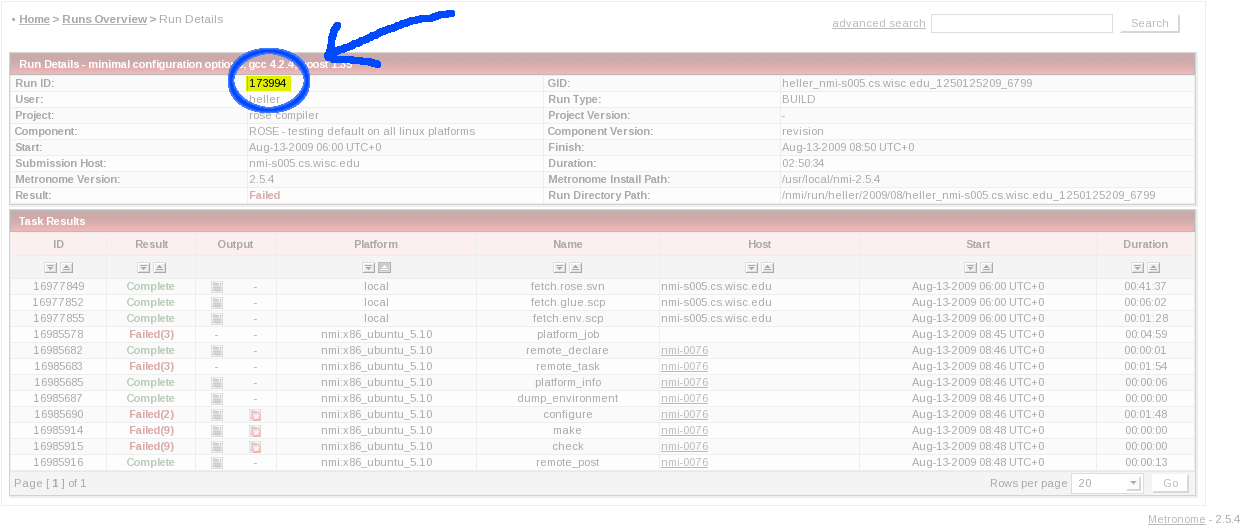
\includegraphics[width=200mm]{nmi-screenshot.png}

	\caption{Example screenshot of a results page, {\tt runid} highlighted.}
	\label{fig:nmi:screenshot}
\end{figure}


{\tt nmi-postmortem} is intended to be run on the submit host.  If it is not in
the {\tt PATH} of the account you are using there, then {\tt scp} the file to
the submit host and place it somewhere in your {\tt PATH}.  If you are using the
shared account, then {\tt nmi-postmortem} should already be in your {\tt PATH}.\\


With this, you can invoke the following on the submit host:\\
\ {\tt nmi-postmortem <runid>}\\


This will do the following:
\begin{itemize}

	\item Determine the machine the test ran on (the {\tt run host}).

	\item Ensure that it is possible to {\tt ssh} to the run host.  This may
	require you entering the account's password a couple of times, but is
	otherwise automated.  This amounts to copying the public key from the submit
    host to the run host's {\tt \$HOME/.ssh/authorized\_keys} file.

	\item Copy {\tt results.tar.gz} to the run machine and extract it there in a
	directory called {\tt run}.  {\bf {\tt WARNING}}: Any previous run directory on
	that machine will be removed first.

	\item {\tt ssh} you onto the run machine, {\tt cd} to the run directory and
	source the environment file for the run.  At this point you should be able
	to investigate in an environment very close to the one the actual run failed
	on.
\end{itemize}

{\tt NOTE}: {\tt nmi-postmortem} invokes {\tt ssh} a lot and assumes that there
exists a file {\tt \$HOME/.ssh/id\_rsa.pub} on the submit host and that this key
has no passphrase.  If this is not the case for the account you are using,
simply invoke {\tt ssh-keygen} and be sure not to specify a passphrase.


\subsection{Default Timeouts}
   See the manual.


\subsection{Where to get help}

\begin{enumerate}
	\item {\bf Mailing Lists} - It is recommended to subscribe to the mailing
		lists listed at \url{http://nmi.cs.wisc.edu/node/521}.  As of this writing,
		these include \tt{uw-nmi-announce} and \tt{nmi-users}.

	\item {\bf Support} - Support's email is {\tt nmi-support@cs.wisc.edu}.

    \item {\bf The Manual} - \url{http://nmi.cs.wisc.edu/node/31}.
\end{enumerate}
%}}}



\section{ROSE API Refactoring}

{\bf This is the outline of the API, add API functions to the next section.}

This a draft design for a new High Level ROSE API where high level function interfaces will be
located that call mechanisms for analysis, transformation, and expected user level support
for ROSE tools. This support is presently spread around in ROSE and this API would
centralize it and make ROSE more clear to users.
There are four levels:
\begin{enumerate}
   \item ROSE Frontend \\
      Generation of Abstract Syntax Tree (AST) from source code or binary executable.
      The AST holds structural representations of the input software.

   \item ROSE Midend \\
      Analysis and transformation support for ROSE-based tools.
   \begin{enumerate}
      \item ROSE Analysis API \\
         This would include intra-procedural analysis, inter-procedural analysis, 
         and whole program analysis (which over comes the issues of separate compilation).
         This analysis can handle either source code analysis, binary analysis, or both.
         Program analysis on source code includes:
         \begin{enumerate}
            \item Program analysis on source code includes:
            \begin{enumerate}
               \item Call Graph Analysis
               \item Class Hierarchy Analysis
               \item Control Flow Analysis
               \item Def-Use Analysis
               \item Dominance Analysis
               \item Dominator Trees And Dominance Frontiers Analysis (old)
               \item Connection of Open Analysis (old)
               \item Pointer Analysis
               \item Procedural Slicing (old; not used) 
               \item Side-Effect Analysis
               \item Value Propagation Analysis
               \item Static Interprocedural Slicing (replaces Procedural Slicing)
               \item Liveness Analysis
               \item Dependence Analysis
               \item AST Interpreter (Interpretation of Concrete Semantics using AST)
            \end{enumerate}
            \item Program analysis on binaries includes:
            \begin{enumerate}
               \item Call graph Analysis
               \item Control Flow Analysis
               \item Constant Propogation
               \item Data Flow Analysis
               \item InstructionSemantics
               \item Library Identification (FLIRT)
               \item Dwarf Debug Format
               \item Analysis of the Binary File Format
            \end{enumerate}
         \end{enumerate}

      \item ROSE Transformation API \\
         Modifications of the AST can be organized as:
         \begin{enumerate}
            \item Instrumentation
            \item Optimization
               These include a range of optimizations relevant for general performance
               optimization of scientific applications.
            \begin{enumerate}
               \item Inlining
               \item Loop optimizations:fusion, fisson, unrolling, blocking, loop
                  interchange, array copy, etc.
               \item Constant Folding
               \item Finite Differencing
               \item Partial Redundancy Elimination
            \end{enumerate}

            \item General Transformations
               These include outlining,
            \begin{enumerate}
               \item Outlining
               \item ImplicitCodeGeneration \\
                  This work makes C++ implicit semantics explicit for C style analysis.
               \item FunctionCallNormalization \\
                  This is a library of function call normizations to support binary
                  analysis.
               \item AST Copy support \\
                  This support permits arbitrary subtrees (or the whole AST) to be copied
                  with control over deep or shallow copying via a single function.
               \item AST Merge support \\
                  This work permits the merging of separate AST's and the sharing of their
                  identically names language declarations to support whole program
                  analysis. Duplicate parts of the merged AST are deleted.
               \item Static Binary Rewriting \\
                  A restricted set of transformations are possible on a binary executable,
                  this section details this work.
            \end{enumerate}
         \end{enumerate}
%        \end{enumerate}

      \item AST Traversals \\
         ROSE provides a number of different techniques to define traversals of the AST
         and associated graphs formed from the AST. 
   \end{enumerate}
%  \end{enumerate}

   \item ROSE Backend \\
      Code generation from the AST (unparsing) and optionally calling the backend
      compiler.  ROSE includes a number of features specific to the code generation phase: 
   \begin{enumerate}
      \item Code generation from arbitrary subtrees of the AST \\
         Users can generate code from subsets of the AST as part of support for custom
         code generation.
      \item Generation of abritrary test with generated code \\
         This section contains the support for the output of arbitrary text as part of the
         generation of code (useful for generating code for specialized GPU tools, etc.).
      \item Code generation Format control \\
         Some control is possible over the formatting of generated code within ROSE.
   \end{enumerate}


   \item ROSE Util \\
      Utility functions useful in ROSE-based tools.
   \begin{enumerate}
      \item AST Visualization \\
         AST support for visualization includes representations as PDF, DOT, and
         a more colorful representation of the whole graph that includes AST plus 
         type attributes (not typically as part of an AST). This work includes
         support for dot2gml translation (in roseIndependentSupport/dot2gml).
         this is where interfaces to possible OGDF (Open Graph Drawing Framework)
         could be put.

      \item AST Query \\
         The AST Query mechanism is a simple approach to getting list of IR nodes.
         It is typically used within analysis or transformations.

      \item AST Consistancy Tests \\
         The consistancy tests validate that the AST is correctly formed. Note that this
         is not a test that the code that will be gnerated is leagal code.

      \item Performance monitoring \\
         This section provides support using in ROSE to measuring both space and 
         time complexity for ROSE based tools.

      \item AST Postprocessing \\
         The AST postprocessing is a step used to fix the AST after some types of 
         modification by the user and to make it a correctly formed AST. Not all
         modifications to the AST can be corrected using this step.

      \item AST File I/O Support \\
         This section contains the support for writing and reading the AST to and from
         files (binary file I/O is used and the design is for performance (both space and
         time)).

      \item Language specific name support \\
         This section contains the support for generating unique names for language
         constructs and handling mangled and unmangled names for use in ROSE based tools.

      \item Support for comments and CPP directives \\
         This section contains the support for reading and writing comments and CPP
         directives within the AST.

      \item GUI Support \\
         This section contains the support for building GUI based tools using ROSE.

      \item Binary Analysis connection to IDA PRO \\
         This section contains the support for using IDA Pro with ROSE for Binary Analysis.

      \item Database Support \\
         This section contains the support for building tools that use SQLite Database.

      \item Graphs and Graph Analysis \\
         This section contains the support for building custom graphs to represent static
         and dynamic ananlysis and graph analysis algorithms to suport of analysis of
         these graphs.

      \item Performance Metric Annotation \\
         This section contains the support for dynamically derived information to be
         written into the AST (performance inforamtion to support analysis and
         optimization tools).

      \item Abstract Handles \\
         This section contains the support for building abstract handles into source code.
         This work is used in the autotuning and also other tools that pass references to
         source code as part of an interface.

      \item Macro Rewrapper \\
         This is currently in the ROSE/projects directory and should perhaps be a part of
         the ROSE API.

      \item Command-line processing support \\
         This is the command line handling used internally by ROSE and made available 
         so that users can process the command line for their specific ROSE based tools.

      \item Common string support \\
         These function support common operations on strings used within ROSE and 
         useful within ROSE-based tools.

      \item Common file and path support \\
         This is a collection of function useful for handling directory structures within
         ROSE-based tools.

      \item Miscellaneous Support \\
         Output of useage information, ROSE version number support, etc.

   \end{enumerate}

\end{enumerate}


% Put onto a new page for development
\newpage

% Blue Book (reference to legendary PDF documentation)
% http://www-cdf.fnal.gov/offline/PostScript/BLUEBOOK.PDF

\section{ROSE API (PUT YOUR LISTS OF FUNCTIONS HERE)}

    This is a group effort to define a better set of high level documents for ROSE
that will explain what is in ROSE at a high level and what users need to know about the
ROSE API and a moderate level of detail.  Only functionality expected to be useful to the
development of ROSE based tools by external users are presented.  Lower level details are
available in other documentation or via the doxygen generated documentation.

Some helpful notes, other ideas, issues, etc.:
\begin{enumerate}
   \item Class-based \\
	It seems that interfaces are more useful if we place them in a
	class rather than a namespace.

   \item Virtual vs. not-virtual \\
	Except where performance is an issue, it's useful to have
	mostly virtual methods.

   \item Namespace \\
	The ROSE API should be in a "rose" namespace which all of our
	source files each import.

   \item Naming style \\
	Agree on style. Most of ROSE uses SomeClass for classes and
	someMethod for methods and functions.

   \item Macros \\
	Header file macros should all be the same form, such as
	ROSE\_WHATEVER\_H.  Feature macros should use a common form
	(perhaps ROSE\_HAS\_WHATEVER or ROSE\_USES\_WHATEVER). Function
	like macros should be replaced with inline functions. Value
	macros should be replaced with static const data members.

   \item Who manages pointed-to memory \\
	Classes with pointers should have a clear statement of who
	manages the pointed-to memory: the class or the caller. Also,
	if the caller manages memory then when can the caller delete
	that memory (must it wait until the object that uses it is
	deleted or did the object make a copy)?

   \item Include files \\
   \fixme{DQ has a bias toward a single rose.h since it avoids bugs due to different orderings of includes.}
	Must the end user include all of rose (rose.h) in order to use
	a particular class?  Our compiling would be *so*much*faster*
	if each file included only what it actually used. (We could
	still have a "rose.h"-like file that includes everything for
	the lazy end user.)

   \item Some provision for header/library consistency \\
	For instance, certain functions in the HDF5 API (like H5\_init()
	that initializes the library) pass a version number from a
	header file that gets compared with a version number compiled
	into the library. If they don't match then there will probably
	be runtime issues and HDF5 can report this before the user
	gets a core dump.  ROSE could do something similar.

   \item Namespace aliases can be used to provide alternative shorter
   namespace names for users, so we can focus on having names that are
   as clear as possible.
\end{enumerate}

Outline where to put list of functions/functionality for each category of the API.

\subsection{Story Of ROSE (JK)}
   This is a section that Jeff Keasler has specific ideas about how to write and
for which he will provide an outline to start the process.

% This is email from Jeff Keasler which I have copied out and put here so
% that we can have one place to look at it.  It is not included into the 
% document (notice that it is commented out).
\commentout{
Getting Started With ROSE

Introduction -- 4 to 7 (single sided) pages
   ROSE is a tool to convert human readable programs into
   data structures that are easily manipulated with algorithms.

   ROSE can help you analyse or transform your software.

      Analysis tasks include:
         Security Analysis
            Code conformance
            Bug Checking
         Dependency Analysis
            Control Flow
            Data Flow

      Transformation tasks include:
         Optimization
         Instrumentation
         Automatic parallelization

   Applications based on ROSE are formally called ``translators''.

   Structure of a ROSE translator
      frontend(argc, argv)
      commandline
      analysis/transformation
      AstTests::runAllTests(project);
      backend(project)

   The Fundamental data structure in ROSE is the AST
       Single expression (a = b + c) displayed as an AST (dot file diagram).
       A group of statements within a scope as represented within the AST.



Reference -- about 30 to 40 pages.

   AST IR Nodes

      Introduction
         What is an IR Node (with example nodes mentioned)?
         Naming and usage (SgXXXXX, isSgxxxxx)?

         Hello world ---  a translator that produces a dot file.

         Output to help you work with the AST
            Dot
            Pdf

      Basic properties
         Parent
         Children
         Scope
         Attributes
         SG_File_Info
         node->sage_class_name()

      Common Operations on an IR Node.
         Insert/delete/modify
            High/Mid/Low level
         Find
            AST Query
            SgSymbolTable
         Traversal

      Specializations of SgNode
         SgLocatedNode
         SgSupport
         SgSymbol
         SgType
         SgAsmNode


      Important IR nodes
         SgBasicBlock
         SgStatement
         ...

      For a complete description of all IR Nodes, see doc XXX.

   AST Features

      Special Scopes
         Prepend/Append operations for all scopes
         SgGlobal
         Functions
         NameSpaces
         Classes
         templates

      Types
        Declarations/Parameters create an SgInitialized name
        classes ?
        declaration vs. defining declaration?
        SgModifier, SgTypeModifier,
           SgStorageModifier, SgAccessModifier, SgDeclarationModifier
        working with types
           manipulation
           string representation

      Variables (SgVarRef)
         Scalars
         Arrays
         Classes

      Functions
           Parameters -- SgInitialized Names
              Accessing, creating
           defining delcaration

      Classes (whole separate section needed for classes?)


   Objects and Memory
      By mindful of scope for SgName, because they quickly self destruct.
      Use/Reuse of SgXXX objects on the heap.

   Unparser
      User added annotations

-----------------------------
(possible separate document)

buildinterface
sageinterface

}


\subsection{User API (All)}
{\bf Proposed location of new ROSE API: {\em ROSE/src/API}}

   The ROSE User Application Program Interface (API) is the subset of ROSE that is
typically required by users to write ROSE based applications for the general
processing of software (source code or executable).  Specialized projects may
require deeper levels of the ROSE software than present in this API and many
project may not use but a small part of this API.  This documentation is
to present ROSE at a high level while covering enough detail to make it
clear what different parts of ROSE are available.

   ROSE will soon be represented by a number of namespaces.  The
API will be represented by four namespaces (the Intermediate Representation
is expected to be in its own namespace.  It is not clear if there should
be a single top level namespace or if there should be namespace
aliases that would permit alternative shorter names (an option).



\subsubsection{Frontend (Yi)}
{\bf Interm proposed namespace name: {\em ROSE\_Frontend}} \\
\fixme{Liao will be proposing namespace names for us to agree upon separately.}
    The frontend of ROSE takes the source code or binary executable 
and generates an Abstract Syntax Tree (AST), which for the basis of 
further work. The AST forms a structural representation of the source
code or binary executable.
\fixme{We might discover that the frontend and backend are too simple to 
deserve their own namespaces.}
\begin{enumerate}
   \item {\bf SgProject* frontend (int argc, char** argv);} \\
   Generates an AST represented by the root node ({\em SgProject}) from
   the commandline in the form defined by {\tt main(int argc, char** argv)}.

   \item {\bf SgProject* frontend (const std::vector$<$std::string$>$ \& argv);} \\
   Generates an AST represented by the root node ({\em SgProject}) from
   an alternative representation of the command line more useful when 
   custom command line editing is required by the translator.

   \item {\bf SgProject* frontendShell (int argc, char** argv);} \\
   Generates an AST represented by the root node ({\em SgProject}) from
   the common command line form, but for files that might be conditionally 
   compiled later.

   \item {\bf SgProject* frontendShell (const std::vector$<$std::string$>$ \& argv);} \\
   Generates an AST represented by the root node ({\em SgProject}) from
   the alternative command line form, but for files that might be conditionally 
   compiled later.
\end{enumerate}

\paragraph{Notes from Robb}
\fixme{These might be too low level for the proposed API.}
\begin{enumerate}
	\item Parsing functions \\
   These methods parse a particular entity from a binary file and
   fill in an existing IR node that was recently constructed.
   See parse() methods in src/frontend/ExecFormats/*.C
   \item Disassembly \\
   Disassembling a buffer into a std::map of instructions.  ROSE
   normally calls this automatically, does a little analysis to
   organize instructions into basic blocks and basic blocks into
   functions, and links everything into the AST. However, its
   also useful to call the disassembler explicitly. Disassemblers
   can be specialized by derivation. There's a number of
   functions and full doxygen documentation (the actual functions
   that disassemble a \_single\_ x86, ARM, or PowerPC instruction
   are only lightly documented). \\
   See doxygen for Disassembler class. \\
   See src/frontend/Disassembler/Disassembler.h
\end{enumerate}


\subsubsection{Midend (All)}
{\bf Interm proposed namespace name: {\em ROSE\_Midend}} \\
   The midend of ROSE is typically where the user interacts with the AST
or uses features in ROSE to generate alternative graphs to represent
specific types of program analysis. The midend includes both analysis
and transformation capabilities and is used by the users to build 
custom analyzes and transformations.

\paragraph{Analysis (TP)}
{\bf Interm proposed namespace name: {\em ROSE\_Analysis}} \\
   Analysis within ROSE by definition does not modify the AST structure.
It might add attributes to IR nodes, but it does not change the structure 
of the AST.  In may cases it may generate specific data structures and
separate analysis may traverse these data structures; thus both are covered
separately.

\subparagraph{Construct (TP \& DQ)}
   This covers the construction of various data structures that are part of
specific forms of analysis or are used in subsequent forms of analysis.
We separate out the API that is specific for source code and binary executable.
\begin{enumerate}
   \item Source (TP) \\
   \begin{enumerate}
      \item Call Graph Analysis
      \item Class Hierarchy Analysis
      \item Control Flow Analysis
      \item Def-Use Analysis
      \item Dominance Analysis
      \item Dominator Trees And Dominance Frontiers Analysis (might be old)

      \item Connection of Open Analysis (might be old) \\
      This might be something for Colorado State to comment upon.

      \item Pointer Analysis \\

      \item Procedural Slicing (might be the old version; not used) 

      \item Side-Effect Analysis

      \item Value Propagation Analysis

      \item Static Interprocedural Slicing (replaces Procedural Slicing)
      \item Liveness Analysis
      \item Dependence Analysis
   \end{enumerate}

   \item Binary (DQ) \\
   \fixme{These might be too low level for the proposed API.}
   \begin{enumerate}
      \item Call Graph Analysis \\
      The Partitioner::mark\_call\_targets() computes a call graph
      based on x86 "CALL" and "FARCALL" instructions, but doesn't
      return any useful information (it uses it immediately to
      partition basic blocks into functions).

      \item Control Flow Analysis \\
      The Partitioner::detectBasicBlocks() method computes an
      basic-block level call graph returned as a
      Partitioner::BasicBlockStarts data structure. It looks at all
      instructions that explicitly change the flow of
      control. However, it might backward from what one would
      expect: for every instruction, it records what other
      instructions call that instruction. (It was done this way
      because that's the info that's needed to detect function
      boundaries.)

      \item Constant Propogation \\
      Constant propagation for binaries is in the
      FindConstantsPolicy which is used with instruction
      semantics. This code is not well documented.

      \item Data Flow Analysis \\
      Part of constant propagation.

      \item Dwarf Debug Format \\
      The Dwarf Debug Format structure is automatically constructed 
      as part of reading the binary executable if it is available.
      Command line options to ROSE translators permit optionally 
      skipping the parsing of the Dwarf format.
   \end{enumerate}
\end{enumerate}

\subparagraph{Use (TP \& DQ)}
   The use of the data structures built to some forms of analysis (e.g. call graph)
can be used to support subsequent forms of analysis that operate on the generated
data structures. We separate out the API that is specific for source code and 
binary executable.
\begin{enumerate}
   \item Source (TP) \\
   \begin{enumerate}
      \item AST Interpreter (Interpretation of Concrete Semantics using AST)
   \end{enumerate}

   \item Binary (DQ) \\
   \begin{enumerate}
      \item InstructionSemantics \\
	Implemented in the X86InstructionSemantics class, which
	requires a policy class (such as FindConstantsPolicy) at
	compile time.

	The implementation only supports 32-bit x86 and is not well
	documented.
      
      \item Library Identification (FLIRT) \\
      This has not yet been moved from {\tt developersScratchSpace/Dan/libraryIdentification\_tests}
      to a more useful location in ROSE.  Likely should be put in the {\em midend} as part
      of {\em analysis}.

      \item Analysis of the Binary File Format \\
      This has not yet been moved from {\tt developersScratchSpace/Dan/astEquivalence\_tests}
      to a more useful location in ROSE.  Likely should be put in the {\em midend} as part
      of {\em analysis}.

      \item Dynamic Analysis of Instruction Execution \\
      There are three interfaces:
      \begin{enumerate}
         \item Ptrace: Uses the Unix ptrace() system call to trace over 
               the network a binary executing on a remote linux machine.
         \item Pin: Traces an executable running on the same machine as ROSE.
         \item Ether: Traces an executable running in Windows XP on 
               a Xen virtual machine on the same hardware as ROSE.
      \end{enumerate}

      \item General Dynamic Analysis \\
      Uses Ether/Xen to execute the specimen in Windows XP on a
      virtual machine and adds new SgAsmGenericSections containing
      disassembled instructions to the AST as those areas
      are discovered.  Can then unparse the AST to a new executable.
      {\em This is work in progress.}

      \item Detecting unreferenced regions \\
      Finding what regions of the binary were never referenced
      during parsing.  The binary I/O utilities keep track of
      everything that was read during parsing and this information
      is available through an ExtentMap (see utilities below). The
      inverse of the ExtentMap will show what hasn't been
      referenced.\\
      See doxygen for ExtentMap class.

      \item Basic block detection \\
      Organize instructions into basic blocks.  The Partitioner
      class is reponsible for taking a set of instructions and
      deciding which instructions belong together in a basic
      block. This analysis is normally called automatically by ROSE
      as part of its disassembly procedure, but it's also useful to
      call this explicitly (especially if you also called the
      Disassembler explicitly, since the disassemlber doesn't
      actually put things into basic blocks).
      Fully documented in doxygen. See Partitioner class. \\
      See src/frontend/Disassembler/Partitioner.h

      \item Function boundary detection \\
      Organize basic blocks into functions. The Partitioner class is
      responsible for taking a set of basic blocks and figuring out
      how to organize them into functions. It can look at other
      parts of a binary AST (like symbol tables), is fully
      configurable, and can be specialized by derivation.
      See doxygen for Partitioner class. \\
      See src/frontend/Disassembler/Partitioner.h

   \end{enumerate}
\end{enumerate}

\paragraph{Transformation}
{\bf Interm proposed namespace name: {\em ROSE\_Transformation}} \\
   Transformation by definition modifies the structure of the AST and can be used
to define instrumentation, optimizations, and custom translation.
\subparagraph{Source (L)}
\lstset{language={C++},basicstyle=\small} 
\begin{enumerate}
   \item Instrumentation 
   \fixme{Do we need this section at all? Can be covered in general
   translations}
   \begin{lstlisting}

   /* Instrument(Add a statement, often a function call) into a function right
      before the return points, handle multiple return statements and return
      expressions with side effects. Return the number of statements inserted.
    */
   int instrumentEndOfFunction (SgFunctionDeclaration *func, SgStatement *s);

   /* Instrument(Add a statement, often a function call) into a function at
      the very beginning.  */
   int instrumentBeginOfFunction (SgFunctionDeclaration *func, SgStatement *s);
   \end{lstlisting}
   \item Optimization
         These include a range of optimizations relevant for general performance
         optimization of scientific applications.
   \begin{enumerate}
      \item Inlining
      \begin{lstlisting}
      /* Inline a function call site*/
      bool inlining (SgFunctionCallExp *);

      /* Inline all call sites to a function within a root AST node,
         return the number of call sites being inlined. */
      int inlining (SgNode* root, SgFunctionDeclartion *);

      /* Inline all call sites to a function with a qualified name,
         return the number of call sites being inlined. */
      int inlining (SgNode* root, const std::string &qualified_func_name);

      /*Aggressive inline all call sites whenever possible for an AST,
        return the number of call sites being inlined. */
      int inlining(SgNode* root);

      \end{lstlisting}
      \item Loop optimizations:fusion, fusion, unrolling, blocking, loop
                  interchange, array copy, etc.
Most API functions take SgNode* instead of SgForStatement* to be compatible for both C and Fortran loops.
       \begin{lstlisting}

       //! Normalize a loop, return true if successful
       //! The loop can be either C for loop or Fortran DO loop
       bool loopNormalization (SgNode* loop);

      /* Check if a for-loop has a canonical form, return loop index, 
         bounds, step, body and so on if requested. */
       bool isCanonicalForLoop (SgNode *loop, SgInitializedName **ivar=NULL, 
            SgExpression **lb=NULL, SgExpression **ub=NULL, SgExpression **step=NULL, 
            SgStatement **body=NULL, bool *hasIncrementalIterationSpace=NULL, 
            bool *isInclusiveUpperBound=NULL);

       /* Unroll a target loop with a specified unrolling factor. 
          It handles steps larger than 1 and adds a fringe loop 
          if the iteration count is not evenly divisible by the unrolling factor. */
       bool loopUnrolling (SgNode *loop, size_t unrolling_factor);

       //! Unroll and jam a loop, with a given unrolling factor
       bool loopUnrollAndJam (SgNode *loop, size_t unrolling_factor);

       /*   Tile the n-level (starting from 1) loop of a perfectly nested loop nest 
            using tiling size s. */
       bool loopTiling (SgNode *loopNest, size_t targetLevel, size_t tileSize);

       /* Interchange/permutate a n-level perfectly-nested loop rooted at 'loop' 
          using a lexicographical order number within (0,depth!). */
       bool loopInterchange (SgNode*loop, size_t depth, size_t lexicoOrder);

       /*  Normalize loop init stmt by promoting the single variable declaration statement 
           outside of the for loop header's init statement, e.g. for (int i=0;) becomes 
           int i_x; for (i_x=0;..) and rewrite the loop with the new index variable, 
           if necessary. */
       bool normalizeForLoopInitDeclaration (SgForStatement *loop);

       //! Fuse two loops into one loop, return the fused loop
       SgNode* loopFusion (SgNode* loop1, SgNode* loop2);
      
       /* Loop fission: break a loop into multiple loops */
       std::vector<std::SgNode*> loopFission (SgNode* src_loop);

// TODO array copy 
       \end{lstlisting}
      \item Constant Folding
       \begin{lstlisting}
        /* Constant folding an AST subtree rooted at 'root'. 
          Avoid folding floating point typed expressions 
          by default to ensure accuracy. */
         void constantFolding (SgNode* root, bool foldFloatPoint = false);

       \end{lstlisting}
      \item Finite Differencing  \fixme{what is this?}
       \begin{lstlisting}
       //! Do finite differencing on one expression within one context.
        void doFiniteDifferencingOne(SgExpression* e,
                             SgBasicBlock* root, RewriteRule* rules);
       \end{lstlisting}

      \item Partial Redundancy Elimination
       \begin{lstlisting}
       /* Apply partial redundancy elimination on AST rooted at r*/
       void partialRedundancyElimination(SgNode* r);
       \end{lstlisting}

   \end{enumerate} % end of optimization

   \item General Transformations \\
         These include outlining, AST copy, and AST merge support, etc.
   \begin{enumerate}
      \item Outlining  
\fixme{Discuss setting internal flags and debugging support}
      \begin{lstlisting}
      //! Accept a set of command line options to set internal behaviors
      void commandLineProcessing(std::vector<std::string> &argvList);

      //! Returns true iff the statement is "outlineable."
      //! Print out reasons for s that can not be outlined if 'verbose' is true
      bool isOutlineable (const SgStatement* s, bool verbose = false);

      //! Preprocess a statement for outlining
      SgBasicBlock* preprocess (SgStatement* s);

       //! Outlines the given basic block into a function named 'name'
       Result outlineBlock (SgBasicBlock* b, const std::string& name);

      //! Outline to a new function with the specified name, calling 
      //! preprocessing internally
      Result outline (SgStatement* s, const std::string& func_name);

      //! Stores the main results of an outlining transformation.
      struct Result
      {
        //! The outlined function's declaration and definition.
        SgFunctionDeclaration* decl_;
      
        //! A call statement to invoke the outlined function.
        SgStatement* call_;
      
        //! A SgFile pointer to the newly generated source file containing the
        // outlined function if -rose:outline:new_file is specified (useNewFile==true)
        SgFile* file_;
      }
       \end{lstlisting}

      \item ImplicitCodeGeneration \\
            This work makes C++ implicit semantics explicit for C style analysis.
\fixme{The granularity for transformation targets? flag to ignore headers, other files?}
       \begin{lstlisting}
       //! Make implicit compiler-generated function explicit,
       //  including default constructors, destructors and copy constructors.
       void defaultFunctionGenerator(SgProject *prj);

       //! The same as the above, except that it operates on the file scope
       void defaultFunctionGenerator(SgFile* f);

       //! The same as the above, except that it operates on a target class
       void defaultFunctionGenerator(SgClassDeclaration* c_decl);

       //!Annotates the AST with calls to class destructors whenever objects
       go out of scope.
       void destructorCallAnnotator(SgProject *prj);

       //! Transforms the evaluation of short-circuited expressions to explicitly
       //! evaluate each step.  A prerequisite of destructorCallAnnotator.
       void shortCircuitingTransformation(SgProject *prj);

       \end{lstlisting}
      

      \item FunctionCallNormalization \\
            This is a library of function call normalizations to support binary
            analysis.
       \begin{lstlisting}
       //! Ensure that no statement will have more than one function call
       //! This is to be done by inserting new temporary variables to replace extra calls
        void functionCallNormalization(SgNode* root);

       \end{lstlisting}

      \item AST creation/building \\      
            Build AST pieces, transparently taking care of side effects as much as possible.
           Used to replace the direct call to constructors. 
       \begin{lstlisting}
       //! Type builders
       SgTypeBool * buildBoolType ();
       SgTypeInt * buildIntType ();
       ...
       //! Expression builders
       SgNullExpression *buildNullExpression ();
       SgIntVal *  buildIntVal (int value=0);
       SgVarRefExp * buildVarRefExp (const std::string &varName, 
                                     SgScopeStatement *scope=NULL);
       ...
       //! Statement builders
       SgVariableDeclaration * buildVariableDeclaration (const SgName &name, 
                                  SgType *type, SgInitializer *varInit=NULL, 
                                              SgScopeStatement *scope=NULL);
       SgWhileStmt * buildWhileStmt (SgStatement *condition, SgStatement *body);
       SgClassDeclaration * buildStructDeclaration (const std::string &name, 
                                       SgScopeStatement *scope=NULL); 
       ...

       //! Misc builders
       SgFile * buildFile (const std::string &inputFileName, 
          const std::string &outputFileName, SgProject *project=NULL);
       SgInitializedName * buildInitializedName (const std::string &name, 
                                                  SgType *type);
       ... 
       \end{lstlisting}

      \item AST insert, deletion, move and replacement \\
            Manipulate AST pieces
       \begin{lstlisting}
       PreprocessingInfo * insertHeader (const std::string &filename, 
           PreprocessingInfo::RelativePositionType position=PreprocessingInfo::after, 
           bool isSystemHeader=false, SgScopeStatement *scope=NULL);
       void insertStatement (SgStatement *targetStmt, SgStatement *newStmt, 
            bool insertBefore=true);
       void insertStatementList (SgStatement *targetStmt, 
            const std::vector< SgStatement * > &newStmts, bool insertBefore=true);
       void insertStatementBefore (SgStatement *targetStmt, SgStatement *newStmt);
       void insertStatementAfter (SgStatement *targetStmt, SgStatement *newStmt);
       void appendStatement (SgStatement *stmt, SgScopeStatement *scope=NULL);
       void prependStatement (SgStatement *stmt, SgScopeStatement *scope=NULL);
       ...
       void deepDelete (SgNode *root);
       void deleteAST (SgNode *node);
       void removeStatement (SgStatement *stmt);
       
       ...
       void replaceExpression (SgExpression *oldExp, SgExpression *newExp, 
            bool keepOldExp=false);
       void replaceStatement (SgStatement *oldStmt, SgStatement *newStmt, 
            bool movePreprocessinInfo=false);
       
       void moveStatementsBetweenBlocks (SgBasicBlock *sourceBlock, 
            SgBasicBlock *targetBlock);
       \end{lstlisting}
       \item AST Copy support \\
         This support permits arbitrary subtrees (or the whole AST) to be copied
         with control over deep or shallow copying via a single function.
         \begin{lstlisting}
         SgNode * deepCopyNode (const SgNode *subtree);
         SgNode * shallowCopyNode (const SgNode *subtree);
         template<typename NodeType>
           NodeType * deepCopy (const NodeType *subtree);
         SgExpression * copyExpression (SgExpression *e);
         SgStatement * copyStatement (SgStatement *s);
         \end{lstlisting}

       \item AST Merge support \\
           This work permits the merging of separate AST's and the sharing of their
           identically names language declarations to support whole program
           analysis. Duplicate parts of the merged AST are deleted.
         \begin{lstlisting}
         //! Merge AST tree from multiple files
         void mergeAST( SgProject* project );

         //! Merge AST from mulitple AST binary dump files
         SgProject * mergeAST(std::vector <FILE *> files);
         \end{lstlisting}


       \end{enumerate} % end of general transformation
   \end{enumerate}  % end of transformation

\subparagraph{Binary (DQ)}
\begin{enumerate}
   \item Static Binary Rewriting \\
         A restricted set of transformations are possible on a binary executable.
         Existing work supports moving and/or resizing a section. We don't handle 
         all cases since this is incredibly complicated. \\
         See {\bf SgAsmGenericFile::shift\_extend()}.
\end{enumerate}

\subsubsection{Backend (DQ)}
{\bf Interm proposed namespace name: {\em ROSE\_Backend}} \\
   The backend part of ROSE generates the code and produces a final executable
(just like any other compiler).  Users don't typically work on any aspect of 
the backend; thus is has a simple API.
\begin{enumerate}
   \item {\bf int backend ( SgProject* project, UnparseFormatHelp *unparseFormatHelp = NULL, UnparseDelegate* unparseDelagate = NULL );} \\
   This function generates source code from the AST and calls the backend
   compiler. The integer error code from the backend compiler is returned.
   UnparseFormatHelp permits limited control over the formatting of the 
   generated source code. UnparseDelegate is currently ignored. For binaries,
   this function generates an assembler listing with section information and
   a reassembled binary executable.

   \item {\bf int backendUsingOriginalInputFile ( SgProject* project );} \\
   This is useful as a test code for testing ROSE for use on projects that target Compass or any
   other analysis only tool using ROSE. Called in tests/testAnalysis.C for example.

   \item Assembler \\
   Generating machine code from SgAsmInstruction nodes. The
   Assembler class is reponsible for taking SgAsmInstruction
   nodes and generating machine code, placing the result in a
   buffer.  The assembler can be specialized by derivation.

   Note: currently we only have an x86-64 assembler. The 32-bit
   needs a bit more work.  The x86 assembler is generated
   automatically from the Intel Instruction Set Reference
   documentation and is thus substantially smaller than the x86
   disassembler. \\
   See doxygen Assembler class. \\
   See src/frontend/Disassembler/Assembler.h

   \item Control of Assembler \\
   Various aspects of assembly can be controlled through
   properties of the Assembler object.  For instance, should the
   assembler use smallest possible data encodings or honor the
   sizes of the instruction operands in the AST; should
   instruction prefixes be emitted in the same order and
   cardinality as the original parse, or in the order recommended
   by Intel; etc. \\
   See doxygen Assembler class. \\
   See src/frontend/Disassembler/Assembler.h

\end{enumerate}

\subsubsection{Utility}
{\bf Interm proposed namespace name: {\em ROSE\_Support}} \\
   These features are important to how applications are developed using ROSE.

\paragraph{AST Utility}
   A collection of the utility support in ROSE is specific to the AST and this are 
presented together:
\begin{enumerate}
   \item AST Traversal (Yi)
   \item AST Query (A)
   \item AST Postprocessing (L) \\
         After transformations to the AST, it is frequently required to call a
         standard AST fixup that will fill in missing pieces of the AST and do a few simple
         tests to validate the AST.
         It can also support bottom-up AST construction by patching up symbols, scope information etc.
    
         \begin{lstlisting}
         //! Fixeup missing pieces of the AST
         void AstPostProcessing(SgNode* node);
         
         // Do we want to expose individual fixup to users? 
         // Some examples are given below 

         //! Connect variable reference to the right variable symbols when feasible, 
         //! return the number of references being fixed. 
         int fixVariableReferences (SgNode *root);

         //! Patch up symbol, scope, and parent information when 
         //! a declaration's scope is known. 
         void fixVariableDeclaration (SgVariableDeclaration *varDecl, SgScopeStatement *s);
         void fixClassDeclaration (SgClassDeclaration *classDecl, SgScopeStatement *s);
         void fixNamespaceDeclaration (SgNamespaceDeclarationStatement *decl, SgScopeStatement *s);
         void fixLabelStatement (SgLabelStatement *label_stmt, SgScopeStatement *s);

         \end{lstlisting}

   \item AST Consistency Tests (L) \\
         This is the highest level of internal consistency testing available in ROSE.
         This test is typically run after the frontend processing (by the user) to
         verify a correct AST before midend processing.
         \begin{lstlisting}
        //! Run all known AST consistency tests
         AstTests::runAllTests(SgNode* root); 
        
        //! Do we want to expose individual tests?
        // Derived class vs. a function call 
        // Tests on a tree vs. memory pools
       
         //! Test on memory pools
         AstTests::testUniqueStatementsInScopes(); 

         //! Test on a whole/sub tree
         AstTests::testUniqueStatementsInScopes(SgNode* root); 

         AstTests::testMangledNames();
         AstTests::testMangledNames(SgNode* root);

         AstTests::testCompilerGeneratedNodes();
         AstTests::testCompilerGeneratedNodes(SgNode* root);

         AstTests::testAstCycles();
         AstTests::testTemplates();
         AstTests::testDefiningAndNondefiningDeclarations();
         AstTests::testSymbolTables();
         AstTests::testMemberFunctions();
         AstTests::testExpressionTypes();

         AstTests::testParentPointersInMemoryPool();
         AstTests::testChildPointersInMemoryPool();

         AstTests::testMappingOfDeclarationsToSymbols();
         AstTests::testExpressionLValue();
        //! Test the declarations to make sure that 
        //defining and non-defining appear in the same file
         AstTests::testMultipleFiles();
         AstTests::testTypesInMemoryPool();
         \end{lstlisting}


   \item AST Visualization (DQ) \\
         Visualization of the AST and related graphs generated from program analysis forms
         an approach to both internal debugging and presentation of specific sorts of
         results.
   \begin{enumerate}
      \item {\bf void generatePDF ( const SgProject \& project );} \\
      Generates a PDF file from the AST.

      \item {\bf void generateDOT ( const SgProject \& project, std::string filenamePostfix );} \\
      Generates a DOT file representing the AST (information about types and many IR nodes
      that are considered attributes to AST nodes are not represented).
      The resulting graph is of the input source code excluding header files.
      The result is a tree (formally).

      \item {\bf void generateDOT\_withIncludes ( const SgProject \& project, std::string filenamePostfix );} \\
      Generates a DOT file representing the AST (information about types and many IR nodes
      that are considered attributes to AST nodes are not represented).
      The resulting graph is of the input source code plus all header files (so it can be
      very large). The result is a tree (formally).

      \item {\bf void generateDOTforMultipleFile ( const SgProject \& project, std::string filenamePostfix );} \\
      Generates a DOT file representing the AST (information about types and many IR nodes
      that are considered attributes to AST nodes are not represented).
      The resulting graph is of all of the files specified on the command line.
      The result is a tree (formally).

      \item {\bf void generateAstGraph ( const SgProject* project, int maxSize, std::string filenameSuffix );} \\
      Generates a DOT file representing the AST and includes information about types and many IR nodes
      that are considered attributes to AST nodes are not represented by the other
      functions above. The resulting graph is of all of the files specified on the command line.
      The result is general graph (not a tree) (formally).
 
 By Liao, What about\\
 \lstinline{void generateDOTforWholeAST(const SgProject* project, std::string filenameSuffix, FilterSetting* fs)}.
   \end{enumerate}

   \item AST File I/O Support (T) \\
         This support permits the AST to be written to a file and read in from a file.
         It is useful for assembling the AST from a whole application and many other
         specialized tools.
\end{enumerate}

Other useful utility functions in ROSE 
\begin{enumerate}
   \item Performance monitoring (DQ) \\
   The {\em TimingPerformance} class defines a simple mechanism used throughout ROSE to
   report the execution performance of different parts of the compilation process.
   As a class variables can be generated on the stack (to record the starting time of
   an execution phase and the destructor for the class will record the elapsed time
   of the execution phase.  
   \begin{enumerate}
      \item {\bf TimingPerformance $<$variable name$>$ ( std::string );} \\
      This constructor builds and starts a timer, the descructor is automatically called
      the end of the scope and records the elapsed time.  The data is saved internally and
      output in a final report in either of two forms (using cout or to a file).

      \item {\bf TimingPerformance::generateReport();} \\
      A report is generated at the end of the execution when
      either the last  {\em TimingPerformance} destructor is called of when the 
      report function is called explicitly.

      \item {\bf TimingPerformance::generateReportToFile(project);} \\
      Write the CSV formatted file of performance data (accumulated over multiple runs)
      Execute the function to generate the data into the report fine independent of the 
      level of verbosity specified from the command-line (does no output to cout or cerr).
      This data can be used by a separate program to graph the different times required
      to run different parts of ROSE on a wide range of files.  It is used mostly for
      debugging complexity issues inside the compiler or in user developed tools using 
      ROSE.

      \item {\bf TimingPerformance::set\_project ( SgProject* project );} \\
      If set, the report will be generated upon calling the destructor for
      the {\em TimingPerformance} object. 

   \end{enumerate}

   \item Language specific name support (DQ) \\
         This section contains the support for generating unique names for language
         constructs and handling mangled and unmangled names for use in ROSE based tools.
   \begin{enumerate}
      \item {\bf virtual SgName SgStatment::get\_qualified\_name() const;} \\
       Qualified names provide a more readable for of newarly unique name for constructs.
       This function is implemented on all SgStatment objects.

      \item {\bf virtual SgName SgStatment::get\_mangled\_name() const;} \\
       Mangled name support so that unique names can be generated.

      \item {\bf SgName SgDeclarationStatement::generate\_alternative\_name\_for\_unnamed\_declaration ( SgNode* parent ) const;} \\
      Support for name mangling of unnamed classes embedded in SgVariableDeclaration and SgTypedefDeclaration.

      \item {\bf SgName SgDeclarationStatement::generate\_alternative\_name\_for\_unnamed\_declaration\_in\_scope ( SgScopeStatement* scope ) const;} \\
      Support for generation of names for unnamed declarations in scopes.

   \end{enumerate}

   \item Support for comments and CPP directives (Yi)

   \item GUI Support (JK \& T)

   \item Binary Analysis connection to IDA PRO (A \& T)

   \item Database Support (A)

   \item Graphs and Graph Analysis (T)

   \item Performance Metric Annotation (L)
   namespace \lstinline{PerformanceMetric} \fixme{single or plural form in name convention?}
\begin{lstlisting}
  //! Loads HPCToolkit XML or GNU gprof text profiling data files given on the command-line
  // and create a list of tree representations (called profile trees) for them.
  ProfileTreeList_t loadProfilingFiles(std::vector<std::string>& argvList);

  //! Attach performance metrics from the profile trees to the AST tree.
  void attachMetrics (const ProfileTreeList_t& profiles,
                      SgProject* proj, bool verbose = false);

  //! Propagate specified metrics from statement level to parent scopes 
  // (loop, function, file and project levels)
  void propagateMetrics(SgProject * project, const std::vector<string> metricNames);

  //!Collect metric names from an AST attached with performance metrics
  void collectMetricnames(SgNode* root, std::vector<std::string>& metricNames); 

  //! Get a metric from a SgNode based on its name
  MetricAttr* getMetric(SgNode*, std::string metric_name);


\end{lstlisting}

   \item Abstract Handles (L)\\
     Abstract handles (namespace \lstinline{AbstractHandle}) are used to specify arbitrary language constructs within an application.
     \begin{lstlisting}
     //! Get SgNode from an abstract handle string
     SgNode* getSgNodeFromAbstracthandle(const std::string& s);  

     //! Create an abstract node from a SgNode
     abstract_node * buildAbstractNode(SgNode*);

     //! Create and abstract handle from an abstract node
     abstract_handle* buildAbstractHandle (abstract_node *);

     //! Create an abstract handle from a handle string
     abstract_handle* buildAbstractHandle(std::string handle_string);

     \end{lstlisting}

   \item Macro Rewrapper (A) \\
         This is a feature not yet ready to be a part of the user API in ROSE.

   \item Command line processing support (Yi) \\
   ROSE based tools can add options to their command line or process options of the
   command line.  These function represent command line support for users to detect
   specialized options or manipulate the command line to add options before processing
   using ROSE (by the frontend API).

   \item Common string support (DQ) \\
         These function support common operations on strings used within ROSE and 
         useful within ROSE-based tools.
   \begin{enumerate}
      \item {\bf int ROSE::containsString ( const std::string \& masterString, const std::string \& targetString );} \\
      Returns result (zero or nonzero) based on containment of {\em targetString} in {\em masterString}.
      \fixme{This function might not be significant enough to be in the API.}
   \end{enumerate}

   \item Common file and path support (Yi) \\
   ROSE based tools frequently have to do some simple simple file name handling
   and this API provides simple access to these functions.
   \fixme{These function currently are in the {\bf ROSE} namespace which we would like to eliminate.}
   \begin{enumerate}
      \item {\bf string ROSE::getWorkingDirectory ();} \\
      Returns working directory of ROSE installation, uses call to {\em getcwd()}.

      \item {\bf std::string ROSE::getSourceDirectory ( std::string fileNameWithPath );} \\
      Return the source directory associated with an installation of ROSE.

      \item {\bf string ROSE::getPathFromFileName ( const string fileName );} \\
      Returns the path associated with the input filename string.

      \item {\bf std::string ROSE::stripPathFromFileName ( const std::string \& fileNameWithPath );} \\
      Returns the path associated with the file.

      \item {\bf std::string ROSE::getFileNameWithoutPath ( SgStatement* statementPointer );} \\
      Returns the name of file associated the specific statement of the AST. The returned
      string excludes the files path.

      \item {\bf std::string ROSE::getFileName ( SgLocatedNode* locatedNodePointer );} \\
      Returns the name of file associated the specific statement or expression of the AST.
      The returned string is the absolute path plus file name.
   \end{enumerate}

   \item ExtentMap \\
   A class for keeping track of contiguous regions of an address
   space. Can be used to manage free lists, or keep track what
   parts of a file have been referenced. Similar to std::map but
   having different lookup functions and able to combine adjacent
   regions into single entries in its data structure. \\
   See doxygen ExecMap class. \\
   See src/frontend/ExecFormats/ExecGeneric.C.

   \item Debug dumps \\
   The dump() methods scattered throughout
   src/frontend/ExecFormats/*.C generate human-readable tables
   describing all details of the SgAsm* nodes. They all take the
   same arguments. These are what produce the *.dump files. \\
   See src/frontend/ExecFormats/*.C

   \item String Management \\
   Functions that manage strings that might be stored in various
   kinds of string tables in a binary file.  Modifying strings,
   sharing storage, repacking tables, reallocating individual
   strings, avoidance of certain file regions, etc. \\
   See src/frontend/ExecFormats/ExecGeneric.C

   \item Section I/O \\
   A variety of functions for reading the original content of a
   binary section either by file offset or through a
   MemoryMap. Also functions for writing back to the file. \\
   Defined for SgAsmGenericFile and SgAsmGenericSection. \\
   See src/frontend/ExecFormats/ExecGeneric.C

   \item MemoryMap \\
   A data structure similar to std::map that maps one address
   space into another (typically a virtual memory address space
   into a file address space).  This allows ROSE to create a
   memory address space separate from its own and manage it as a
   program loader would do. \\
   See doxygen MemoryMap class. \\
   See src/frontend/ExecFormats/MemoryMap.h

   \item Data conversion \\
   Functions for converting data from file format to memory
   format. Most of these are to handle byte order, but there are
   some other encodings as well. \\
   See src/frontend/ExecFormats/ExecGeneric.C

   \item Miscellaneous Support (DQ) \\
         Output of usage information, ROSE version number support, etc.
   \begin{enumerate}
      \item {\bf void SgFile::usage ( int status );} \\
      This function reports information about ROSE options.
      \item {\bf std::string version\_message ();} \\
      This function provides a string form of the version message 
      (e.g. output by {\em --version} option in ROSE).
      \item {\bf std::string version\_number ();} \\
      This function provides a string form of the version number of ROSE
      (in the form major.minor.patch).
   \end{enumerate}

\end{enumerate}


\subsection{IR (PC)}
{\bf Interm proposed namespace name: {\em ROSE\_IR}} \\
   The Intermediate Representation (IR) used in ROSE has data types used
within the interfaces of the ROSE API.  An understanding of the ROSE API 
thus requires some familiarity with the hierarchical organization of the 
IR.  However this the IR is perhaps best represented by the Doxygen
generated web pages which present both the hierarchy of C++ classes 
used to represent the IR and the details of the individual classes.

\newpage

% Red Book (reference to legendary PDF documentation)
%  http://www.adobe.com/devnet/postscript/pdfs/PLRM.pdf

\section{ROSE Example Projects}
   These project demonstrate types of tools that have been built using ROSE and are 
small enough to include within the ROSE distribution (taken from the ROSE/projects
directory):
\begin{enumerate}
   \item Compass
   \item Auto Parallelization
   \item Assembly To Source AST
   \item Auto Tuning
   \item Haskell port
   \item Java port
   \item MPI Code Motion
   \item Reverse Computation
   \item Qt Designer Plugins
   \item Distributed Memory Analysis Compass
   \item Name Consistancy Checker
   \item Name Similarities
   \item Run-time Error Detection (RTED)
   \item Mixed Static Dynamic Analysis
   \item Taint Check
   \item UpcTranslation
   \item CERT Secure Code Project
   \item Data-Structure Graphing
   \item Documentation Generator
   \item Bug Seeding
   \item (Review the projects directory)
\end{enumerate}

This work should coinside with tutorial examples
that should the use of the API and present the
simple executables that generated specific 
forms of analysis (e.g. call graph, outliner, etc.).

Topics that it is less clear where to put (or even if
to put) in the ROSE API include:
\begin{itemize}
   \item Annotation Language Parser (annotationLanguageParser directory; not working)
   \item Distributed Memory Analysis (distributedMemoryAnalysis directory)
   \item AST Rewrite Mechanism (supress this from the API for now).
   \item ompLowering (not for the user interface)
   \item OpenMP Reduction Variable Recognition
\end{itemize}
